\chapter{Vector Calculus} \label{Sec:vector}

In Chapter~\ref{Sec:linearAlgebra} we introduced the concept of a vector, without reference to Calculus. Vectors do not only have to consist of scalar values, but may be functions as well. Because of this, it is meaningful to bring in the concepts of Calculus and discuss instantaneous rates of change and integrals of quantities. The study of vector calculus is vital to understanding many area of physics relevant to nuclear engineering including mechanics, fluid dynamics, and electrodynamics. This chapter is separated into two parts: differential and integral vector calculus.

For notation, we define the concept of a \emph{multivariablescalar field} $f(x,y,z)$, which we sometimes write in shorthand as $f(\pos)$ where $\pos = (x,y,z)$. A scalar field takes values of $(x,y,z)$ as input and provides a number as output. Generally speaking, we will use unbolded characters to denote scalar fields or numbers. We can also introduce the concept of a \emph{vector field}
\begin{align}
  \mathbf{F}(x,y,z) = F_x(x,y,z) \ihat + F_y(x,y,z) \jhat + F_z(x,y,z) \khat
\end{align}
that takes values of $(x,y,z)$ as input and returns a vector as output. We will generally use capital bolded letters in this chapter to denote vector fields with components with non-bolded capital letters with subscripts. Constant vectors will generally be given by lowercase bold letters, unless denoted otherwise. In defining these terms, we explicitly used Cartesian coordinates. One of the powerful features of vectors, however, is that they can be written in a manner that is independent of the coordinate system. This chapter will discuss different coordinate systems such as cylindrical and spherical coordinates as well. To this end, this chapter derives the concepts of basis vectors in curvilinear and explains how they are used with coordinate transformations.

In the second part of this chapter, integral vector calculus is discussed. The topics include line, surface, and volume integrals; fundamental theorems of vector calculus including the divergence and Stokes' theorem; and finally we provide an introduction to scalar and vector potential functions.

%%%%%%%%%%%%%%%%%%%%%%%%%%%%%%%%%%%%%%%%%%%%%%%%%%%%%%%%%%%%%%%%%%%%%%%%%%%%%%%%%%%%%%%%%%%%%%%
%%%%%%%%%%%%%%%%%%%%%%%%%%%%%%%%%%%%%%%%%%%%%%%%%%%%%%%%%%%%%%%%%%%%%%%%%%%%%%%%%%%%%%%%%%%%%%%
\section{Vector Derivatives}

First, we will study the methods of assessing different rates of change of vector fields. In addition to the standard total and partial derivatives, we also have an operator called a gradient that converts a scalar field into a vector field. We can also apply this gradient on vector fields using the multiplication operations of dot products, cross products, and outer products to produce different quantities with different physical meanings. 

%%%%%%%%%%%%%%%%%%%%%%%%%%%%%%%%%%%%%%%%%%%%%%%%%%%%%%%%%%%%%%%%%%%%%%%%%%%%%%%%%%%%%%%%%%%%%%%
\subsection{Derivative of a Vector Field}

The derivative of a vector field is the simplest of the operations, being the simple distribution of the derivative of each component. The derivative of a vector field with respect to some parameter $t$ is
\begin{align}
  \dho{\mathbf{F}}{t} &= \dho{F_x}{t} \ihat + \dho{F_y}{t} \jhat + \dho{F_z}{t} \khat.
\end{align}
The parameter $t$ could be one of the position variables $(x,y,z)$ as well.

%%%%%%%%%%%%%%%%%%%%%%%%%%%%%%%%%%%%%%%%%%%%%%%%%%%%%%%%%%%%%%%%%%%%%%%%%%%%%%%%%%%%%%%%%%%%%%%
\subsection{Gradient}

The gradient operator in Cartesian coordinates is defined as
\begin{align}
  \nabla = \dho{}{x} \ihat + \dho{}{y} \jhat + \dho{}{z} \khat .
\end{align}
Normally the gradient operator acts upon scalar field $f(x,y,z)$ and outputs a vector field $\mathbf{F}(x,y,z)$:
\begin{align}
  \mathbf{F} = \nabla f = \dho{f}{x} \ihat + \dho{f}{y} \jhat + \dho{f}{z} \khat .
\end{align}
The vector described by the vector $\nabla f$ at each point $(x,y,z)$ points along the direction of steepest ascent.

\begin{figure}[!tb]
\begin{center}

\begin{subfigure}[b]{0.3\textwidth}
  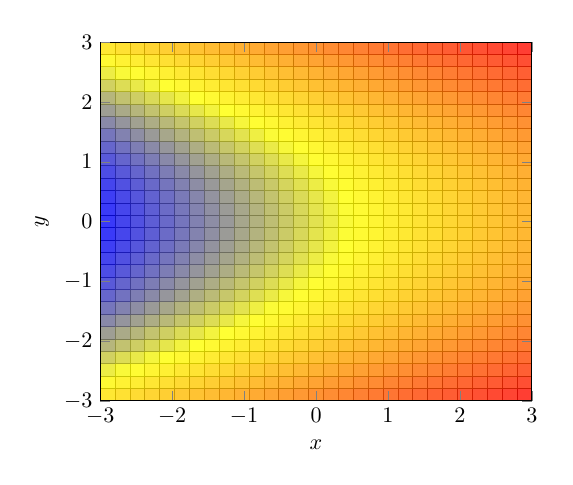
\begin{tikzpicture}[scale=0.8] \begin{axis}[xlabel=$x$,ylabel=$y$,view={0}{90}]
  \addplot3[
    surf,
    opacity=0.8,
    samples=30, samples y=30,
    domain=-3:3,domain y=-3:3
  ]
  {2*x + y*y - 1};
  \end{axis}
  \end{tikzpicture}
\end{subfigure}
\hspace{2cm}
\begin{subfigure}[b]{0.3\textwidth}
  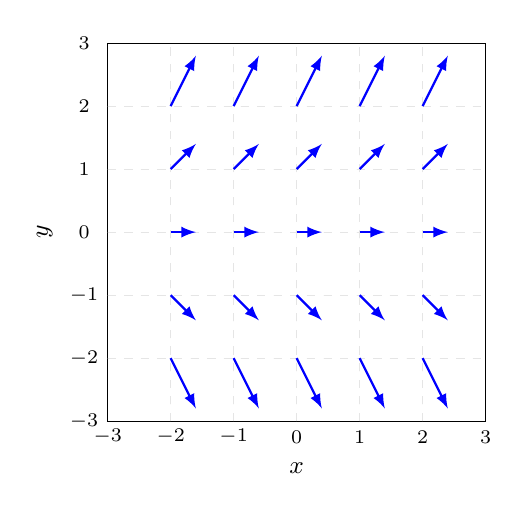
\begin{tikzpicture}[scale=0.8]
  \draw (-3,-3) -- (3,-3) -- (3,3) -- (-3,3) -- cycle;
  \node at (0,-3.75) {\small $x$};
  \node[rotate=90] at (-4,0) {\small $y$};
  \foreach \x in {-2,-1,0,1,2} 
      \foreach \y in {-2,-1,0,1,2} 
        { 
          \draw[dashed,color=gray!20] (\x,-3) -- (\x,3);
          \draw[dashed,color=gray!20] (-3,\y) -- (3,\y);
        } 

  \foreach \x in {-3,-2,-1,0,1,2,3}
     \node at (\x,-3.25) {\scriptsize $\x$};
  \foreach \y in {-3,-2,-1,0,1,2,3} 
      \node at (-3.375,\y) {\scriptsize $\y$};

  \foreach \x in {-2,-1,0,1,2} 
      \foreach \y in {-2,-1,0,1,2} 
        { 
          \draw[-latex,thick,blue] (\x,\y) -- ({\x + 0.4},{\y + 0.4*\y }); 
        } 
  \end{tikzpicture}
\end{subfigure}

\caption{Depiction of a scalar field $f(x,y) = 2x + y^2 - 1$ and its associated gradient vector field.}
\label{Fig:vector_gradientExample}
\end{center}
\end{figure}


An example of the gradient for a 2-D scalar field $f(x,y) = 2x + y^2$ is shown in Fig.~\ref{Fig:vector_gradientExample}. The color plot provides the scalar field where the blue values denote negative scalar values of the field and red denote positive values. When the gradient is applied, we get $\nabla f = 2 \ihat + 2y \jhat$, a vector field, denoted by the arrow plot on the right. At each coordinate, a vector is given with a relative (not absolute) magnitude and an orientation. As we can see, along the $x$ axis, the gradient points only along the $x$-axis, denoting that it is the direction of steepest ascent. Off the $x$ axis, the gradient points away from the origin, denoting that the direction of steepest ascent is at some angle.

%%%%%%%%%%%%%%%%%%%%%%%%%%%%%%%%%%%%%%%%%%%%%%%%%%%%%%%%%%%%%%%%%%%%%%%%%%%%%%%%%%%%%%%%%%%%%%%
\subsection{Directional Derivative}

Sometimes we are interested in the instantaneous rate of change of a scalar field along a particular direction. For this purpose, we define the directional derivative:
\begin{align}
  \nabla_\mathbf{v} f = \mathbf{v} \cdot \nabla f.
\end{align}
This gives the instantaneous rate of the function $f(x,y,z)$ moving through some point $(x,y,z)$ with a ``velocity'' vector $\mathbf{v}$. The directional derivative takes a scalar field and returns another scalar field.

It is often the case that the vector $\mathbf{v}$ is a unit vector $\dir$. We also sometimes write the directional derivative as
\begin{align}
  \frac{df}{ds} = \dir \cdot \nabla f,
\end{align}
where $s$ is a coordinate axis defined along the direction unit vector $\dir$.

We can show that the gradient gives the vector of steepest ascent by taking the directional derivative with the unit vector $\dir$:
\begin{align}
  \dir \cdot \nabla f = | \dir | | \nabla f | \cos \theta = | \nabla f | \cos \theta .
\end{align}
Note that $| \dir | = 1$ since $\dir$ is a unit vector. The directional derivative is maximized where $\cos \theta = 1$.
\begin{align}
  \dir \cdot \nabla f = | \nabla f | . \nonumber
\end{align}
This occurs when the unit vector is the normalized gradient
\begin{align}
  \dir = \frac{ \nabla f }{ | \nabla f | } .
\end{align}
Therefore, the directional derivative is maximized along the gradient.

%%%%%%%%%%%%%%%%%%%%%%%%%%%%%%%%%%%%%%%%%%%%%%%%%%%%%%%%%%%%%%%%%%%%%%%%%%%%%%%%%%%%%%%%%%%%%%%
\subsection{Divergence}

We can take the dot product of the gradient operator with a vector field. In Cartesian coordinates, the divergence of a vector field is defined as
\begin{align}
  \nabla \cdot \mathbf{F} = \dho{F_x}{x} + \dho{F_y}{y} + \dho{F_z}{z}.
\end{align}
The divergence operator takes a vector field and returns a scalar field as output.

The motivation for applying the divergence operator is that it has the physical significance of being the density of the flux of a vector field out of some differential volume at each point $(x,y,z)$. In other words, the divergence is a local measure of the net outward flow of a vector field. 

In the context of fluid dynamics, flows with fluid velocity $\mathbf{u}$ for which $\nabla~\cdot~\mathbf{u} = 0$ are called incompressible. In this case, the velocity field vector points are not allowed to point toward or away from one another, as it would involve the fluid becoming more or less dense. In the context of electromagnetism, the magnetic field follows $\nabla~\cdot~\mathbf{B} = 0$, which is referred to as a solenoidal field. The divergence gives information about how much each point in space behaves like a localized source of a field. Since there are no point sources of magnetic field (called magnetic monopoles), no point behaves like a localized point source and therefore the magnetic field exhibits no divergence.

%%%%%%%%%%%%%%%%%%%%%%%%%%%%%%%%%%%%%%%%%%%%%%%%%%%%%%%%%%%%%%%%%%%%%%%%%%%%%%%%%%%%%%%%%%%%%%%
\subsection{Curl}

The curl is the cross product of the gradient operator and a vector field. In Cartesian coordinates this is given as
\begin{align}
  \nabla \times \mathbf{F} &= 
  \left| \begin{array}{c c c}
  \ihat & \jhat & \khat \\
  \dho{}{x} & \dho{}{y} & \dho{}{z} \\
        F_x &       F_y &       F_z \\ \end{array} \right| \nonumber \\
  &= \left( \dho{F_z}{y} - \dho{F_y}{z} \right) \ihat 
   - \left( \dho{F_z}{x} - \dho{F_x}{z} \right) \jhat
   + \left( \dho{F_y}{x} - \dho{F_x}{y} \right) \khat .
\end{align}
The curl takes a vector field and returns another vector field.

The curl of a vector field describes the local circulation of a vector field about each point $(x,y,z)$. One can envision an infinitesimal surface about each point $(x,y,z)$ with an outward normal vector oriented such that the direction of rotation is clockwise with respect to that vector, which is $\nabla \times \mathbf{F}$. The magnitude of the curl gives a measure of the degree of circulation.

In fluid dynamics, the curl is used to measure the vorticity of the flow, which is the rate that the fluid rotates at a given point. For this reason, we often refer to fluid flows where $\nabla \times \mathbf{F} = \mathbf{0}$ as irrotational. Later, we will see that when the curl of a force field is zero, we can call that force conservative and the work done by such a force along a trajectory only depends upon the endpoints. This is important, because the fundamental forces of nature (e.g., gravity) are conservative, even though macroscopic descriptions of nature used in engineering include nonconservative forces such as friction or viscosity.

%%%%%%%%%%%%%%%%%%%%%%%%%%%%%%%%%%%%%%%%%%%%%%%%%%%%%%%%%%%%%%%%%%%%%%%%%%%%%%%%%%%%%%%%%%%%%%%
\subsection{Convective (Material) Derivative}

In fluid dynamics, we often consider a fixed differential element of fluid with scalar property $f(x,y,z,t)$ (e.g., the concentration of some radioisotope tracer) moving in a velocity field $\mathbf{u}(x,y,z,t)$. This is described by the convective or material derivative:
\begin{align}
  \frac{Df}{Dt} = \dho{f}{t} + \mathbf{u} \cdot \nabla f .
\end{align}

We can also define the convective derivative for a vector field $\mathbf{F}$ (e.g., the fluid momentum) as well:
\begin{align}
  \frac{D\mathbf{F}}{Dt} = \dho{\mathbf{F}}{t} + \mathbf{u} \cdot \nabla \mathbf{F} .
\end{align}
The first term is simply the derivative of a vector field. The second term, however, involves taking the gradient of a vector field. This may be defined using the outer product. For Cartesian coordinates, this is
\begin{align}
  \nabla \mathbf{F} &= \nabla \otimes \mathbf{F}
  = \left( \dho{}{x} \ihat + \dho{}{y} \jhat + \dho{}{x} \khat \right) \otimes \bigg( F_x \ihat + F_y \jhat + F_z \khat \bigg) .
\end{align}
Expanding the outer product gives
\begin{align}
  \nabla \mathbf{F} 
  &= \dho{F_x}{x} \ihat \ihat + \dho{F_y}{x} \ihat \jhat + \dho{F_z}{x} \ihat \khat \nonumber \\
  &+ \dho{F_x}{y} \jhat \ihat + \dho{F_y}{y} \jhat \jhat + \dho{F_z}{y} \jhat \khat \nonumber \\
  &+ \dho{F_x}{z} \khat \ihat + \dho{F_y}{z} \khat \jhat + \dho{F_z}{z} \khat \khat .
\end{align}
Taking the dot product with the fluid velocity gives
\begin{align}
  \mathbf{u} \cdot \nabla \mathbf{F} 
  &= u_x \left( \dho{F_x}{x} \ihat + \dho{F_y}{x} \jhat + \dho{F_z}{x} \khat \right) \nonumber \\
  &+ u_y \left( \dho{F_x}{y} \ihat + \dho{F_y}{y} \jhat + \dho{F_z}{y} \khat \right) \nonumber \\
  &+ u_z \left( \dho{F_x}{z} \ihat + \dho{F_y}{z} \jhat + \dho{F_z}{z} \khat \right) .
\end{align}
Combining the vector components yields
\begin{align}
  \mathbf{u} \cdot \nabla \mathbf{F} 
  &= \left( u_x \dho{F_x}{x} + u_y \dho{F_x}{y} + u_z \dho{F_x}{z} \right) \ihat \nonumber \\
  &+ \left( u_x \dho{F_y}{x} + u_y \dho{F_y}{y} + u_z \dho{F_y}{z} \right) \jhat \nonumber \\
  &+ \left( u_x \dho{F_z}{x} + u_y \dho{F_z}{y} + u_z \dho{F_z}{z} \right) \khat .
\end{align}
Putting this altogether the convective derivative expressed as components becomes
\begin{align}
  \frac{D\mathbf{F}}{Dt} 
  &= \left( \dho{F_x}{t} + u_x \dho{F_x}{x} + u_y \dho{F_x}{y} + u_z \dho{F_x}{z} \right) \ihat \nonumber \\
  &+ \left( \dho{F_y}{t} + u_x \dho{F_y}{x} + u_y \dho{F_y}{y} + u_z \dho{F_y}{z} \right) \jhat \nonumber \\
  &+ \left( \dho{F_z}{t} + u_x \dho{F_z}{x} + u_y \dho{F_z}{y} + u_z \dho{F_z}{z} \right) \khat .
\end{align}

%%%%%%%%%%%%%%%%%%%%%%%%%%%%%%%%%%%%%%%%%%%%%%%%%%%%%%%%%%%%%%%%%%%%%%%%%%%%%%%%%%%%%%%%%%%%%%%
\subsection{Laplacian}

We can also take second derivatives using the vector operations. The most common and useful of these is the divergence of the gradient, or the Laplacian. In Cartesian coordinates, the Laplacian of a scalar field (the scalar Laplacian) is given by
\begin{align}
  \nabla \cdot \nabla f = \nabla^2 f = 
  \frac{\partial^2 f}{ \partial x^2 } + \frac{\partial^2 f}{ \partial y^2 } + \frac{\partial^2 f}{ \partial z^2 } .
\end{align}
The Laplacian of a scalar field is another scalar field.

The Laplacian measures how a quantity given by a scalar field $f$ spreads out from a point $(x,y,z)$. The Laplacian is commonly encountered in problems related to diffusion, which describe heat conduction and neutrons diffusion. Related to the scalar Laplacian is the diffusion operator, which is
\begin{align}
  \nabla \cdot D(\pos) \nabla,
\end{align}
where $D(\pos)$ is a \emph{diffusion coefficient} that may be a function of position. Where $D(\pos) = D = \text{constant}$, the diffusion operator takes the form of the generic scalar Laplacian multiplied by the constant diffusion coefficient.

In addition to being able to take the Laplacian of a scalar field, we may also take the Laplacian of a vector field $\nabla \cdot \nabla \mathbf{F}$. As we saw when discussing the convective derivative, we must take the gradient of a vector field, which, for Cartesian coordinates, is 
\begin{align}
  \nabla \mathbf{F} 
  &= \dho{F_x}{x} \ihat \ihat + \dho{F_y}{x} \ihat \jhat + \dho{F_z}{x} \ihat \khat \nonumber \\
  &+ \dho{F_x}{y} \jhat \ihat + \dho{F_y}{y} \jhat \jhat + \dho{F_z}{y} \jhat \khat \nonumber \\
  &+ \dho{F_x}{z} \khat \ihat + \dho{F_y}{z} \khat \jhat + \dho{F_z}{z} \khat \khat . \nonumber
\end{align}
Next, taking the divergence gives
\begin{align}
  \nabla \cdot \nabla \mathbf{F} 
  &= \dhotwo{F_x}{x} \ihat + \dhotwo{F_y}{x} \jhat + \dhotwo{F_z}{x} \khat \nonumber \\
  &+ \dhotwo{F_x}{y} \ihat + \dhotwo{F_y}{y} \jhat + \dhotwo{F_z}{y} \khat \nonumber \\
  &+ \dhotwo{F_x}{z} \ihat + \dhotwo{F_y}{z} \jhat + \dhotwo{F_z}{z} \khat .
\end{align}
Collecting the different terms
\begin{align}
  \nabla \cdot \nabla \mathbf{F} 
  &= \left( \dhotwo{F_x}{x} + \dhotwo{F_x}{y} + \dhotwo{F_x}{z} \right) \ihat \nonumber \\
  &+ \left( \dhotwo{F_y}{x} + \dhotwo{F_y}{y} + \dhotwo{F_y}{z} \right) \jhat \nonumber \\
  &+ \left( \dhotwo{F_z}{x} + \dhotwo{F_z}{y} + \dhotwo{F_z}{z} \right) \khat . 
\end{align}
This can now be written in terms of the scalar Laplacian:
\begin{align}
  \nabla^2 \mathbf{F} = \nabla^2 F_x \ihat + \nabla^2 F_y \jhat + \nabla^2 F_z \khat .
\end{align}
This shows that for Cartesian coordinates the vector Laplacian is a sum of the scalar Laplacian of each component and describes how much each component of the vector field $\mathbf{F}$ spreads out from $(x,y,z)$.

An important identity that generalizes the vector Laplacian to any coordinate system is
\begin{align}
  \nabla^2 \mathbf{F} = \nabla ( \nabla \cdot \mathbf{F} ) - \nabla \times ( \nabla \times \mathbf{F} ).
\end{align}
In other words, the vector Laplacian is the gradient of the divergence minus the curl of the curl. There are other combinations of second derivatives that appear throughout the application of vector calculus, but these will not be discussed in detail here.

%%%%%%%%%%%%%%%%%%%%%%%%%%%%%%%%%%%%%%%%%%%%%%%%%%%%%%%%%%%%%%%%%%%%%%%%%%%%%%%%%%%%%%%%%%%%%%%
\subsection{Vector Derivative Identities}

There are numerous vector identities that can be employed to manipulate equations and cast them in simpler or more physically meaningful forms.

Two common vector identities for vector fields $\mathbf{A}$, $\mathbf{B}$, and $\mathbf{C}$ are as follows: The first involve interchanging the vectors when we take dot product of the cross product of vectors:
\begin{align}
  \mathbf{A} \cdot ( \mathbf{B} \times \mathbf{C} ) = \mathbf{B} \cdot ( \mathbf{C} \times \mathbf{A} ) = \mathbf{C} \cdot ( \mathbf{A} \times \mathbf{B} ) .
\end{align}
The three vectors can be reordered in a cyclic manner. 

The second vector identity that simplifies the cross product of the cross product is
\begin{align}
\mathbf{A} \times ( \mathbf{B} \times \mathbf{C} ) = \mathbf{B} ( \mathbf{A} \cdot \mathbf{C} ) - \mathbf{C} ( \mathbf{A} \cdot \mathbf{B} ) .
\end{align}
This allows for the expression of the cross products in terms of dot products. Note that this vector identity is often referred to be its mnemonic, the BAC-CAB identity, which follows the ordering of the vectors on the right-hand side.

We can also write six different product rules involving the gradient, divergence, and curl. The gradient of the product of two scalar fields $f$ and $g$ has a similar form as the standard product rule:
\begin{align}
  \nabla ( f g ) = f \nabla g + g \nabla f.
\end{align}
The gradient of the dot product of two vector fields $\mathbf{A}$ and $\mathbf{B}$ is
\begin{align}
  \nabla ( \mathbf{A} \cdot \mathbf{B} ) = 
  \mathbf{A} \times ( \nabla \times \mathbf{B} ) + \mathbf{B} \times ( \nabla \times \mathbf{A} ) 
  + ( \mathbf{A} \cdot \nabla ) \mathbf{B} + ( \mathbf{B} \cdot \nabla ) \mathbf{A}.
\end{align}
The divergence of the product of a scalar field $\mathbf{f}$ and vector field $\mathbf{A}$ is
\begin{align}
  \nabla \cdot ( f \mathbf{A} ) = f ( \nabla \cdot \mathbf{A} ) + \mathbf{A} \cdot \nabla f .
\end{align}
The divergence of the cross product of two vector fields $\mathbf{A}$ and $\mathbf{B}$ is
\begin{align}
  \nabla \cdot ( \mathbf{A} \times \mathbf{B} ) = \mathbf{B} \cdot ( \nabla \times \mathbf{A} ) - \mathbf{A} \cdot ( \nabla \times \mathbf{B} ) .
\end{align}
The curl of the product of a scalar field $\mathbf{f}$ and vector field $\mathbf{A}$ is
\begin{align}
  \nabla \times ( f \mathbf{A} ) = f ( \nabla \times \mathbf{A} ) - \mathbf{A} \times ( \nabla f ) .
\end{align}
Finally, the curl of the cross product of two vector fields $\mathbf{A}$ and $\mathbf{B}$ is
\begin{align}
  \nabla \times ( \mathbf{A} \times \mathbf{B} ) = (
  \mathbf{B} \cdot \nabla ) \mathbf{A} - ( \mathbf{A} \cdot \nabla ) \mathbf{B} + \mathbf{A} ( \nabla \cdot \mathbf{B} ) - \mathbf{B} ( \nabla \cdot \mathbf{A} ) .
\end{align}

Additionally, there are identities involving the second derivatives. The first is that the divergence of the curl is zero
\begin{align}
  \nabla \cdot ( \nabla \times \mathbf{A} ) = 0.
\end{align}
The curl of the gradient is also zero
\begin{align}
  \nabla \times ( \nabla \mathbf{A} ) = \mathbf{0}.
\end{align}
Finally, we can rearrange the definition of the vector Laplacian to get the curl of the curl as
\begin{align}
   \nabla \times ( \nabla \times \mathbf{A} ) = \nabla ( \nabla \cdot \mathbf{A} ) - \nabla^2 \mathbf{A}.
\end{align}

Finally, we can list identities for third derivatives, i.e., those involving the Laplacian. The gradient of the scalar Laplacian can be written as the vector Laplacian of the gradient
\begin{align}
  \nabla ( \nabla^2 f ) = \nabla^2 ( \nabla f ).
\end{align}
The divergence of vector Laplacian is the scalar Laplacian of the divergence
\begin{align}
  \nabla \cdot ( \nabla^2 \mathbf{A} ) = \nabla^2 ( \nabla \cdot \mathbf{A} ).
\end{align}
Finally, the curl of the vector Laplacian is the vector Laplacian of the curl
\begin{align}
  \nabla \times ( \nabla^2 \mathbf{A} ) = \nabla^2 ( \nabla \times \mathbf{A} ).
\end{align}

%%%%%%%%%%%%%%%%%%%%%%%%%%%%%%%%%%%%%%%%%%%%%%%%%%%%%%%%%%%%%%%%%%%%%%%%%%%%%%%%%%%%%%%%%%%%%%%
\subsection{Example: Vorticity Equation for an Incompressible Fluid}

An incompressible fluid satisfies a simplified version of the Navier-Stokes equation:
\begin{align}
  \rho \frac{D\mathbf{u}}{Dt} = -\nabla p + \mu \nabla^2 \mathbf{u}.
\end{align}
Here $\mathbf{u}(x,y,z,t)$ is the fluid velocity vector field, $p$ is the scalar pressure field, $\rho$ is the constant fluid density, and $\mu$ is the constant fluid viscosity. Since the fluid is incompressible, we know that the divergence of the fluid velocity field is zero,
\begin{align}
  \nabla \cdot \mathbf{u} = 0.
\end{align}
We define the vorticity as the curl of the velocity field,
\begin{align}
  \boldsymbol\omega = \nabla \times \mathbf{u}.
\end{align}
The vorticity, as the name implies, describes the local circulation of the fluid. 

The goal is to derive a conservation equation for the vorticity. To begin, we first expand the convective derivative:
\begin{align}
  \rho \frac{D\mathbf{u}}{Dt} = \rho \dho{\mathbf{u}}{t} + \rho \mathbf{u} \cdot \nabla \mathbf{u} =  -\nabla p + \mu \nabla^2 \mathbf{u}.
\end{align}
Recall the vector identity for the gradient of a dot product of two vector fields:
\begin{align}
  \nabla ( \mathbf{A} \cdot \mathbf{B} ) = 
  \mathbf{A} \times ( \nabla \times \mathbf{B} ) + \mathbf{B} \times ( \nabla \times \mathbf{A} ) 
  + ( \mathbf{A} \cdot \nabla ) \mathbf{B} + ( \mathbf{B} \cdot \nabla ) \mathbf{A}. \nonumber
\end{align}
Here we let $\mathbf{A} = \mathbf{B} = \mathbf{u}$ to get
\begin{align}
  \nabla ( \mathbf{u} \cdot \mathbf{u} ) = 2 \mathbf{u} \times ( \nabla \times \mathbf{u} ) + 2 ( \mathbf{u} \cdot \nabla ) \mathbf{u} .
\end{align}
Solving for $\mathbf{u} \cdot \nabla \mathbf{u}$:
\begin{align}
  ( \mathbf{u} \cdot \nabla ) \mathbf{u} = \frac{1}{2} \nabla ( \mathbf{u} \cdot \mathbf{u} ) - \mathbf{u} \times ( \nabla \times \mathbf{u} ).
\end{align}
Inserting this into the fluid differential equation gives
\begin{align}
  \rho \dho{\mathbf{u}}{t} + \frac{\rho}{2} \nabla ( \mathbf{u} \cdot \mathbf{u} ) - \rho \mathbf{u} \times ( \nabla \times \mathbf{u} ) =  -\nabla p + \mu \nabla^2 \mathbf{u}.
\end{align}
Note that the term
\begin{align}
  \frac{\rho}{2} \nabla ( \mathbf{u} \cdot \mathbf{u} ) \nonumber
\end{align}
is related to the kinetic energy of the fluid.

Next, we take the curl of the resulting equation to get:
\begin{align}
  \rho \dho{\mathbf{\boldsymbol\omega}}{t} + \frac{\rho}{2} \nabla \times \nabla ( \mathbf{u} \cdot \mathbf{u} ) - \rho \nabla \times ( \mathbf{u} \times \boldsymbol\omega ) =  -\nabla \times \nabla p + \mu \nabla \times ( \nabla^2 \mathbf{u} ).
\end{align}
Because the curl of the gradient is zero, we can eliminate the kinetic energy and pressure terms:
\begin{align}
  \rho \dho{\mathbf{\boldsymbol\omega}}{t} - \rho \nabla \times ( \mathbf{u} \times \boldsymbol\omega )  =  \mu \nabla \times ( \nabla^2 \mathbf{u} ).
\end{align}
We can apply the identity for the curl of the cross product:
\begin{align}
  \nabla \times ( \mathbf{u} \times \boldsymbol\omega ) = 
  ( \boldsymbol\omega \cdot \nabla ) \mathbf{u} - ( \mathbf{u} \cdot \nabla ) \boldsymbol\omega + \mathbf{u} ( \nabla \cdot \boldsymbol\omega ) - \boldsymbol\omega ( \nabla \cdot \mathbf{u} ) .
\end{align}
The third term is zero because the divergence of the curl is zero
\begin{align}
   \nabla \cdot \boldsymbol\omega =  \nabla \cdot ( \nabla \times \mathbf{u} ) = 0.
\end{align}
The fourth term is zero because the fluid is incompressible. Therefore, we now have
\begin{align}
  \rho \dho{\mathbf{\boldsymbol\omega}}{t} + \rho ( \mathbf{u} \cdot \nabla ) \boldsymbol\omega - \rho ( \boldsymbol\omega \cdot \nabla ) \mathbf{u}  =  \mu \nabla \times ( \nabla^2 \mathbf{u} ).
\end{align}
The first two terms can be regrouped into the convective derivative of the vorticity. For the right-hand side, we can equate the curl of the vector Laplacian with the Laplacian of the curl:
\begin{align}
  \nabla \times ( \nabla^2 \mathbf{u} ) = \nabla^2 ( \nabla \times \mathbf{u} ) = \nabla^2 \boldsymbol\omega .
\end{align}
The vorticity equation becomes
\begin{align}
  \frac{D \boldsymbol\omega }{ Dt } = ( \boldsymbol\omega \cdot \nabla ) \mathbf{u} + \frac{\mu}{\rho} \nabla^2 \boldsymbol\omega .
\end{align}
The equation states that the change of the vorticity of a fluid element is given by the stretching of the vortex because of gradients in the flow velocity and is dissipated by the viscosity of the fluid.


%%%%%%%%%%%%%%%%%%%%%%%%%%%%%%%%%%%%%%%%%%%%%%%%%%%%%%%%%%%%%%%%%%%%%%%%%%%%%%%%%%%%%%%%%%%%%%%
%%%%%%%%%%%%%%%%%%%%%%%%%%%%%%%%%%%%%%%%%%%%%%%%%%%%%%%%%%%%%%%%%%%%%%%%%%%%%%%%%%%%%%%%%%%%%%%
\section{Curvilinear Coordinates}

In calculus we are permitted to have basis vectors that are continuous functions of space. This allows us to define useful coordinate systems that make solving practical engineering problems much simpler. The most common of these are curvilinear coordinates. In 2-D the most common curvilinear coordinate system is polar coordinates, where the basis vectors in $(x,y)$ are replaced with radial and polar angle basis vectors $(r,\theta)$. In 3-D, we have two common curvilinear coordinate systems. The first is cylindrical coordinates $(r,\theta,z)$ with radial, polar, and axial variables and spherical basis vectors. The second is spherical coordinates $(r,\theta,\phi)$ with radial, polar, and azimuthal basis vectors respectively. This section reviews these coordinate systems. In this section we will also show the that basis vectors can be expressed as partial derivatives.


%%%%%%%%%%%%%%%%%%%%%%%%%%%%%%%%%%%%%%%%%%%%%%%%%%%%%%%%%%%%%%%%%%%%%%%%%%%%%%%%%%%%%%%%%%%%%%%
\subsection{Cartesian Basis Vectors}

To begin, we start with Cartesian coordinates. Here we will show the results in 2D, as it is easier to visualize graphically, but the results easily extend to 3D. Let us consider some position vector
\begin{align}
  \mathbf{R}(x,y) = x \ihat + y \jhat .
\end{align}
Additionally, we have the position vector evaluated at $\mathbf{R}(x + \Delta x, y)$ for some offset $\Delta x$ while $y$ is left constant. $\mathbf{R}(x + \Delta x, y)$ is shifted in the $x$ direction by $\Delta x$. Next, we define a vector as the difference of these $\mathbf{R}(x + \Delta x, y) - \mathbf{R}(x,y)$. These vectors are illustrated in Fig.~\ref{Fig:vector_illustrationOfDerivative_Cartesian}.

\begin{figure}[htb!]
\begin{center}
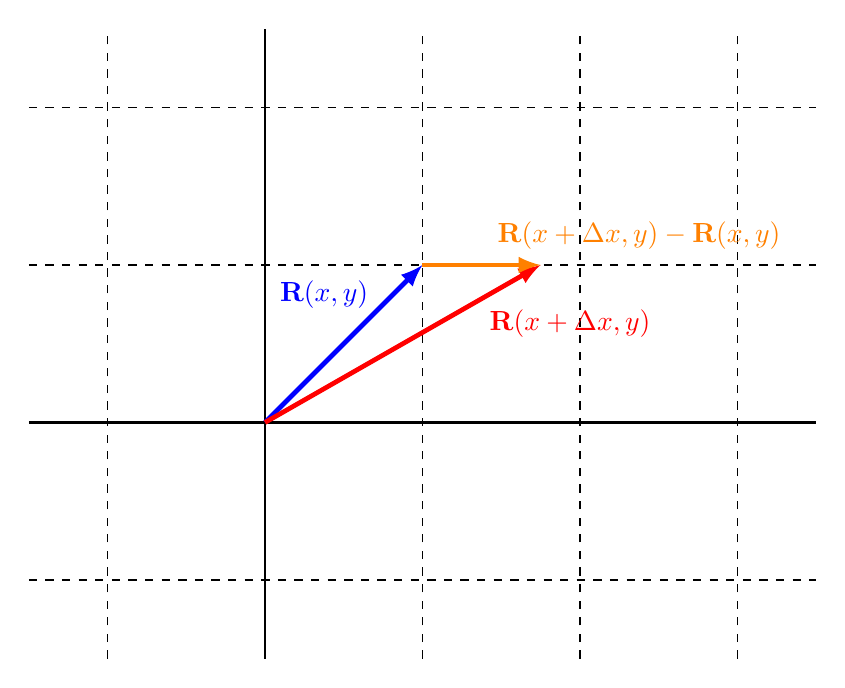
\begin{tikzpicture}
%  \fill[color=blue!20,opacity=0.5] (0,0) -- (2,0) -- (2,2) -- (0,2) -- cycle;
%  \fill[color=red!20,opacity=0.5]  (0,0) -- (4,2) -- (6,0) -- (2,-2) -- cycle;
  \draw[thick] (-3,0) -- (7,0);
  \draw[thick] (0,-3) -- (0,5);
  \foreach \x in {-2,0,2,4,6}
    \draw[dashed] (\x,-3) -- (\x,5);
  \foreach \y in {-2,0,2,4}
    \draw[dashed] (-3,\y) -- (7,\y);

  \draw[-latex,line width=0.6mm,color=blue] (0,0) -- (2,2);
  \node[color=blue] at (0.75,1.625) {$\mathbf{R}(x,y)$};

  \draw[-latex,line width=0.6mm,color=red] (0,0) -- (3.5,2);
  \node[color=red] at (3.875,1.25) {$\mathbf{R}(x+\Delta x,y)$};  
  
  \draw[-latex,line width=0.6mm,color=orange] (2,2) -- (3.5,2);
  \node[color=orange] at (4.75,2.375) {$\mathbf{R}(x+\Delta x,y) - \mathbf{R}(x,y)$};  
\end{tikzpicture}
\caption{Illustration of derivative along $x$ direction.}
\label{Fig:vector_illustrationOfDerivative_Cartesian}
\end{center}
\end{figure}

The derivative is then
\begin{align}
  \dho{\mathbf{R}}{x} \approx \frac{ \mathbf{R}(x + \Delta x, y) - \mathbf{R}(x,y) }{ \Delta x } .
\end{align}
The magnitude of the vector $\mathbf{R}(x + \Delta x, y) - \mathbf{R}(x,y)$ is $\Delta x$. Therefore, the magnitude of the derivative is one. Then the limit gives a unit vector in the $x$ direction:
\begin{align}
   \dho{\mathbf{R}}{x} = \lim_{\Delta x \rightarrow 0} \frac{ \mathbf{R}(x + \Delta x, y) - \mathbf{R}(x,y) }{ \Delta x } 
   =  \lim_{\Delta x \rightarrow 0} \frac{ \Delta x \ihat}{ \Delta x } = \ihat = \mathbf{e}_x.
\end{align}
By similar arguments, a small change in $y$ gives
\begin{align}
   \dho{\mathbf{R}}{y} = \lim_{\Delta y \rightarrow 0} \frac{ \mathbf{R}(x, y + \Delta y ) - \mathbf{R}(x,y) }{ \Delta y } 
   =  \lim_{\Delta y \rightarrow 0} \frac{ \Delta x \jhat}{ \Delta x } = \jhat = \mathbf{e}_y.
\end{align}
Likewise, in 3-D, a small change in $z$ gives
\begin{align}
   \dho{\mathbf{R}}{z} = \lim_{\Delta z \rightarrow 0} \frac{ \mathbf{R}(x, y, z + \Delta z ) - \mathbf{R}(x,y,z) }{ \Delta z } 
   = \lim_{\Delta z \rightarrow 0} \frac{ \Delta z \khat}{ \Delta z } = \khat = \mathbf{e}_z .
\end{align}

%%%%%%%%%%%%%%%%%%%%%%%%%%%%%%%%%%%%%%%%%%%%%%%%%%%%%%%%%%%%%%%%%%%%%%%%%%%%%%%%%%%%%%%%%%%%%%%
\subsection{Polar Basis Vectors}

In 2-D we often analyze problems with circular symmetry, and in these cases polar coordinates are ideal. Rather than describe the coordinates using $x$ and $y$ positions, we instead use the distance from the origin, the radius $r$, and some angle with respect to the $x$ axis, the polar angle $\theta$. The radial coordinate has a range of $[0,\infty)$ and the polar angle coordinate has a range of $[0,2\pi)$. The relationships to go from Cartesian to polar coordinates are
\begin{subequations}
\begin{align}
  r &= \sqrt{ x^2 + y^2 }, \\
  \theta &= \tan^{-1} \left( \frac{y}{x} \right) ;
\end{align}
\end{subequations}
and the conversions from polar to Cartesian coordinates are
\begin{subequations}
\begin{align}
  x &= r \cos \theta , \\
  y &= r \sin \theta .
\end{align}
\end{subequations}

To get the basis vectors we do similar to what we did for Cartesian coordinates, but using a position vector $\mathbf{R}(r,\theta)$. For the radial coordinate, we have vectors $\mathbf{R}(r,\theta)$ and $\mathbf{R}(r + \Delta r, \theta)$. As before, we take the difference between the two $\mathbf{R}(r + \Delta r, \theta) - \mathbf{R}(r,\theta)$ and observe that its magnitude is $\Delta r$. Taking the limit, we get the same result as with Cartesian coordinates:
\begin{align}
   \dho{\mathbf{R}}{r} = \lim_{\Delta r \rightarrow 0} \frac{ \mathbf{R}(r + \Delta r, \theta ) - \mathbf{R}(r,\theta) }{ \Delta r } = 
   = \lim_{\Delta r \rightarrow 0} \frac{ \Delta r \rhat}{ \Delta r } = \rhat = \mathbf{e}_r .
\end{align}
An aspect of $\mathbf{e}_r = \rhat$ is that, unlike the Cartesian basis vector, it always points away from the origin, and therefore depends explicitly on the $\theta$ coordinate.

\begin{figure}[tb!]
\begin{center}
\begin{tikzpicture}
  \foreach \r in {2.5, 5} 
     \draw[dashed] (0,0) circle (\r);
  \foreach \t in {0, 30, 60, 90, 120, 150, 180, 210, 240, 270, 300, 330}
     \draw[dashed] (0,0) -- ({7*cos(\t)},{7*sin(\t)});

  \draw[-latex,line width=0.6mm,color=blue] (0,0) -- ({2.5*cos(30)},{2.5*sin(30)});
  \draw[-latex,line width=0.6mm,color=red] (0,0) -- ({2.5*cos(75)},{2.5*sin(75)});
  \draw[-latex,line width=0.6mm,color=orange] ({2.5*cos(30)},{2.5*sin(30)}) -- ({2.5*cos(75)},{2.5*sin(75)});  
    
  \node[color=magenta,fill=white] at ({3.75*cos(70)},{3.75*sin(70)}) {$\mathbf{e}_\theta$}; 
  \node[color=magenta,fill=white] at ({4.75*cos(35)},{4.75*sin(35)}) {$\mathbf{e}_r$}; 
  \draw[-latex,,line width=0.6mm,color=magenta] ({2.5*cos(30)},{2.5*sin(30)}) -- +({2.5*cos(120)},{2.5*sin(120)});
  \draw[-latex,,line width=0.6mm,color=magenta] ({2.5*cos(30)},{2.5*sin(30)}) -- +({2.5*cos(30)},{2.5*sin(30)});
  
  \node[color=blue,fill=white] at ({1.75*cos(15) + 0.5},{1.75*sin(15)}) {$\mathbf{R}(r,\theta)$};
  \node[color=red, fill=white]  at ({1.75*cos(120) - 0.125},{1.75*sin(120) + 0.25}) {$\mathbf{R}(r,\theta + \Delta \theta)$};

  \draw[-latex,line width=0.6mm,color=blue] (0,0) -- ({3.75*cos(180)},{3.75*sin(180)});
  \draw[-latex,line width=0.6mm,color=red] (0,0) -- ({3.75*cos(225)},{3.75*sin(225)});
  \draw[-latex,line width=0.6mm,color=orange] ({3.75*cos(180)},{3.75*sin(180)}) -- ({3.75*cos(225)},{3.75*sin(225)}); 

  \node[color=magenta,fill=white] at ({5.75*cos(183.5)},{5.75*sin(183.5)}) {$\mathbf{e}_r$}; 
  \node[color=magenta,fill=white] at ({5.25*cos(218.5)},{5.25*sin(218.5)}) {$\mathbf{e}_\theta$}; 
  \draw[-latex,,line width=0.6mm,color=magenta] ({3.75*cos(180)},{3.75*sin(180)}) -- +({3.75*cos(270)},{3.75*sin(270)}); 
  \draw[-latex,,line width=0.6mm,color=magenta] ({3.75*cos(180)},{3.75*sin(180)}) -- +({2.5*cos(180)},{2.5*sin(180)});
\end{tikzpicture}
\caption{Illustration of radial and polar unit vectors $\mathbf{e}_r$ and $\mathbf{e}_\theta$ for two different radii and polar angles, but same $\Delta \theta$.}
\label{Fig:vector_illustrationOfDerivative_Polar}
\end{center}
\end{figure}

For the polar basis vector, we take the position vectors $\mathbf{R}(r, \theta)$ and $\mathbf{R}(r, \theta + \Delta \theta)$. These two vectors are illustrated in blue and red respectively in Fig.~\ref{Fig:vector_illustrationOfDerivative_Polar} for two different sets with the same $\Delta \theta$ but different radii. The difference between the two is given in the same plot in orange. To find the magnitude of the difference vector $\ell = | \mathbf{R}(r, \theta + \Delta \theta) - \mathbf{R}(r, \theta) |$, we can use the law of cosines
\begin{align}
  \ell^2 = r^2 + r^2 - 2rr\cos( \Delta \theta ) = 2r^2 [ 1 - \cos( \Delta \theta ) ].
\end{align}
Since $\Delta \theta$ is small, we can approximate it with a Taylor series expansion about $\Delta \theta = 0$:
\begin{align}
  \cos( \Delta \theta ) \approx \cos(0) - \Delta \theta \sin(0) - \frac{ ( \Delta \theta )^2 }{2} \cos(0)
  = 1 - \frac{ ( \Delta \theta )^2 }{2} .
\end{align}
Substituting this expansion into the law of cosines
\begin{align}
  \ell^2 \approx 2r^2 [ 1 - ( 1 - \frac{ ( \Delta \theta )^2 }{2} ) ] = r^2 ( \Delta \theta )^2, \quad \ell \approx r \Delta \theta .
\end{align}
Note that the magnitude of the difference is proportional to the radius $r$. Also observe that the difference vector for a finite $\Delta \theta$ is not tangent to the radial coordinate; however, as $\Delta \theta$ becomes smaller the difference vector becomes increasingly tangent and limits to a vector as such. The limit as $\Delta \theta$ goes to zero is
\begin{align}
   \dho{\mathbf{R}}{\theta} = \lim_{\Delta \theta \rightarrow 0} \frac{ \mathbf{R}(r, \theta + \Delta \theta ) - \mathbf{R}(r,\theta) }{ \Delta \theta } 
   =  \lim_{\Delta \theta \rightarrow 0} \frac{ r \Delta\theta \thetahat}{\Delta\theta} 
   = r \thetahat = \mathbf{e}_\theta .
\end{align}
Here we note that, unlike for the Cartesian or radial basis vectors, the unit polar basis vector $\thetahat$ is not the same as the unnormalized polar basis vector $\mathbf{e}_\theta$, with the difference being a factor of the radius. Here $\mathbf{e}_\theta$ scales in proportion to the radius. We use both basis vectors here because each has a particular value depending upon the application.

%%%%%%%%%%%%%%%%%%%%%%%%%%%%%%%%%%%%%%%%%%%%%%%%%%%%%%%%%%%%%%%%%%%%%%%%%%%%%%%%%%%%%%%%%%%%%%%
\subsection{Cylindrical Basis Vectors}

We now proceed to the 3-D coordinate systems. The first is cylindrical coordinates, which, as the name implies is useful for problems that have cylindrical characteristics. Similar to the polar coordinate system, we have a radial coordinate $r$, polar angle coordinate $\theta$, and, now in addition, an axial coordinate $z$. The radial coordinate has a range of $[0,\infty)$, the polar angle coordinate has a range of $[0,2\pi)$, and the axial coordinate ranges from $(-\infty,\infty)$. Note that some mathematics textbooks use different symbols for these coordinate variables; here we have chosen the most common convention used in physics.

The coordinate transformations are almost identical to polar coordinates except for the addition of the axial coordinate, which is just the $z$ coordinate in Cartesian coordinates. The transformation for Cartesian to cylindrical is
\begin{subequations}
\begin{align}
  r &= \sqrt{ x^2 + y^2 }, \\
  \theta &= \tan^{-1} \left( \frac{y}{x} \right) , \\
  z &= z.
\end{align}
\end{subequations}
and the conversions from polar to Cartesian coordinates are
\begin{subequations}
\begin{align}
  x &= r \cos \theta , \\
  y &= r \sin \theta , \\
  z &= z .
\end{align}
\end{subequations}

The basis vectors are largely identical to the polar coordinate system with the axial coordinate behaving identically to the Cartesian coordinate basis vector. For completeness, these are
\begin{subequations}
\begin{align}
  \dho{\mathbf{R}}{r} &= \rhat = \mathbf{e}_r, \\
  \dho{\mathbf{R}}{\theta} &= r \thetahat = \mathbf{e}_\theta, \\ 
  \dho{\mathbf{R}}{z} &= \zhat = \mathbf{e}_z.
\end{align}
\end{subequations}
Here we use $\zhat$ instead of $\khat$ to distinguish between the use of cylindrical coordinates versus Cartesian coordinates; however, they are, for all purposes, identical.

%%%%%%%%%%%%%%%%%%%%%%%%%%%%%%%%%%%%%%%%%%%%%%%%%%%%%%%%%%%%%%%%%%%%%%%%%%%%%%%%%%%%%%%%%%%%%%%
\subsection{Spherical Basis Vectors}

The other 3-D curvilinear coordinate that is common is the spherical coordinate system. The spherical coordinate system has a radial coordinate $r$, a polar angle coordinate $\theta$ that moves along a line of constant longitude from the north to south pole, and azimuthal angle $\phi$ that moves eastward along a line of constant latitude around the sphere. Note that radial coordinate goes from $[0,\infty)$, the polar angle coordinate goes from $[0,\pi]$, and the azimuthal angle coordinate goes from $[0,2\pi)$. As with the cylindrical coordinate system, we are using the most common convention used in physics, which differs from many mathematical texts.

The coordinate transformation rules from Cartesian to spherical coordinates are
\begin{subequations}
\begin{align}
  r &= \sqrt{ x^2 + y^2 + z^2 } , \\
  \theta &= \cos^{-1} \left( \frac{z}{ \sqrt{ x^2 + y^2 + z^2 } } \right), \\
  \phi &= \tan^{-1} \left( \frac{y}{x} \right) .
\end{align}
\end{subequations}
The transformation rules from spherical to Cartesian coordinates are
\begin{subequations}
\begin{align}
  x &= r \sin \theta \cos \phi , \\
  y &= r \sin \theta \sin \phi, \\
  z &= r \cos \theta .
\end{align}
\end{subequations}


The radial basis vector is identical to the polar and cylindrical coordinates:
\begin{subequations}
\begin{align}
  \dho{\mathbf{R}}{r} &= \rhat = \mathbf{e}_r.
\end{align}
The polar angle in spherical coordinates has a different range, but the polar basis vector is identical to its analogs in polar and cylindrical coordinates:
\begin{align}
  \dho{\mathbf{R}}{\theta} &= r \thetahat  = \mathbf{e}_\theta .
\end{align}
To derive the azimuthal basis vector, we again take a position vector $\mathbf{R}(r,\theta,\phi)$ and compare it to another position vector with azimuthal offset $\Delta \phi$ for fixed radial coordinate $r$ and polar angle coordinate $\theta$, $\mathbf{R}(r,\theta,\phi + \Delta \phi)$. We then have to consider how the length of the difference $\mathbf{R}(r,\theta,\phi + \Delta \phi) - \mathbf{R}(r,\theta,\phi)$ scales with $r$ and $\theta$. As $r$ changes, the circumference of the circular path of constant latitude grows in proportion to the radius, so the magnitude of the difference scales in direct proportion to $r$, which is the same as the polar coordinate. For variable polar angle $\theta$, however, the circumference also changes. Near the north pole, the distance around the sphere along a line of constant latitude is shorter than near the equator. Therefore, for a fixed azimuthal offset $\Delta \phi$, we travel proportionately further near the equator than near the poles. Doing a bit of trigonometry can show that the circumference is proportional to $\sin \theta$. Therefore, the azimuthal basis vector is
\begin{align}
  \dho{\mathbf{R}}{\phi} &= r \sin \theta \phihat  = \mathbf{e}_\phi .
\end{align}
\end{subequations}

A note about all of the major coordinate systems---Cartesian, polar, cylindrical, and spherical---are orthogonal, and, if the unit basis vectors are used, orthonormal. The coordinate systems are defined such that at any position all of the coordinate basis vectors are always oriented such that they are 90$^\circ$ from each other. 

This completes our discussion of the major coordinate systems used in a large majority of scientific and engineering applications. There are other coordinate systems that are occasionally used for specialized applications including ellipsoidal and toroidal coordinate systems; however, given that they are seldom encountered, they will not be discussed here.


%%%%%%%%%%%%%%%%%%%%%%%%%%%%%%%%%%%%%%%%%%%%%%%%%%%%%%%%%%%%%%%%%%%%%%%%%%%%%%%%%%%%%%%%%%%%%%%
%%%%%%%%%%%%%%%%%%%%%%%%%%%%%%%%%%%%%%%%%%%%%%%%%%%%%%%%%%%%%%%%%%%%%%%%%%%%%%%%%%%%%%%%%%%%%%%
\section{Coordinate Transformations}

In the context of linear algebra we discussed the concept of changing a basis. A change of basis takes a set of basis vectors, which define a coordinate system, and transforms them into a new set of basis vectors, which define a new coordinate system. Recall that we developed a transformation matrix $\mathbf{T}$ and the basis vectors transformed covariantly with respect to themselves (the definition of a coordinate transformation), whereas components of a vector in one coordinate system transform contravariantly using $\mathbf{T}^{-1}$ with respect to the basis vectors.

%%%%%%%%%%%%%%%%%%%%%%%%%%%%%%%%%%%%%%%%%%%%%%%%%%%%%%%%%%%%%%%%%%%%%%%%%%%%%%%%%%%%%%%%%%%%%%%
\subsection{Jacobian and Transformation Matrix}

The Jacobian matrix provides a method of changing basis vectors from one coordinate system to another and is directly analogous to the transformation matrices from linear algebra. Because we saw in the previously that the basis vectors are described by partial derivatives, we can use the chain rule from multivariable calculus to relate them. In 2-D Cartesian to polar we have:
\begin{subequations}
\begin{align}
  \dho{\mathbf{R}}{r} &= \dho{x}{r} \dho{\mathbf{R}}{x} + \dho{y}{r} \dho{\mathbf{R}}{y} , \\
  \dho{\mathbf{R}}{\theta} &= \dho{x}{\theta} \dho{\mathbf{R}}{x} + \dho{y}{\theta} \dho{\mathbf{R}}{y} .
\end{align}
\end{subequations}
Equivalently,
\begin{subequations}
\begin{align}
  \evec_r &= \dho{x}{r} \evec_x + \dho{y}{r} \evec_y , \\
  \evec_\theta &= \dho{x}{\theta} \evec_x + \dho{y}{\theta} \evec_y.
\end{align}
\end{subequations}
Since the transformations of $x = r \cos \theta$ and $y = r \sin \theta$ are given, we can explicitly evaluate the derivatives to obtain
\begin{subequations}
\begin{align}
  \evec_r &= \cos \theta \evec_x + \sin \theta \evec_y , \\
  \evec_\theta &= -r \sin \theta \evec_x + r \cos \theta \evec_y.
\end{align}
\end{subequations}
Since a vector is a column vector in matrix notation, we can express the transformation matrix with columns corresponding to those vectors,
\begin{align}
  \mathbf{J} = \frac{ \partial ( x, y ) }{ \partial ( r, \theta ) } =
   \left[ \begin{array}{c c}
   \cos \theta &  -r \sin \theta \\
   \sin \theta &   r \cos \theta \\ \end{array} \right] =
   \left[ \begin{array}{c c}
   \rfrac{x}{r} & -y \\
   \rfrac{y}{r} &  x \\ \end{array} \right] .
\end{align}
Here we used the symbol $\mathbf{J}$ as opposed to $\mathbf{T}$. Sometimes the notation of a partial derivative of multiple arguments with respect to multiple arguments is used as well to explicitly specify the coordinate transform performed by the matrix. This matrix is called the \emph{Jacobian matrix} that transforms the basis vectors from Cartesian to polar coordinates in terms of $\evec_r$ and $\evec_\theta$. The Jacobian matrix is also used to derive the expressions for length, area, and volume, which will be discussed later in this chapter. 

Recall that the unit vector $\evec_\theta$ is unnormalized, and therefore increases in magnitude in proportion to the distance from the origin. It is often more convenient to transform to a coordinate system where the basis vectors are unnormalized. Recall $\evec_r = \rhat$ and $\evec_\theta = r \thetahat$; the basis unit vectors of the polar coordinate system become is
\begin{subequations}
\begin{align}
  \rhat &= \cos \theta \ihat + \sin \theta \jhat , \\
  \thetahat &= -\sin \theta \ihat + \cos \theta \jhat.
\end{align}
\end{subequations}
This gives the transformation matrix
\begin{align}
  \mathbf{T} =
   \left[ \begin{array}{c c}
   \cos \theta &  -\sin \theta \\
   \sin \theta &   \cos \theta \\ \end{array} \right] =
   \left[ \begin{array}{c c}
   \rfrac{x}{r} & -\rfrac{y}{r} \\
   \rfrac{y}{r} &  \rfrac{x}{r} \\ \end{array} \right] .
\end{align}



Obtaining the Jacobian matrix to convert from Cartesian to cylindrical coordinates is largely identical, so this is given as
\begin{align}
  \mathbf{J} = \frac{ \partial ( x, y, z ) }{ \partial ( r, \theta, z) } =
   \left[ \begin{array}{c c c}
   \cos \theta & -r \sin \theta & 0 \\
   \sin \theta &  r \cos \theta & 0 \\ 
             0 &            0 & 1 \\ \end{array} \right] =
   \left[ \begin{array}{c c c}
   \rfrac{x}{r} & -y & 0 \\
   \rfrac{y}{r} &  x & 0 \\
              0 &  0 & 1 \\ \end{array} \right] .
\end{align}
As with polar coordinates, the Jacobian matrix transforms into a coordinate system with an unnormalized basis vector $\evec_\theta$. To get the more conventional unit basis vectors $(\rhat, \thetahat, \zhat)$ we use the following transformation matrix:
\begin{align}
  \mathbf{T} = 
   \left[ \begin{array}{c c c}
   \cos \theta & -\sin \theta & 0 \\
   \sin \theta &  \cos \theta & 0 \\ 
             0 &            0 & 1 \\ \end{array} \right] =
   \left[ \begin{array}{c c c}
   \rfrac{x}{r} & -\rfrac{y}{r} & 0 \\
   \rfrac{y}{r} &  \rfrac{x}{r} & 0 \\
              0 &             0 & 1 \\ \end{array} \right] .
\end{align}

To go from Cartesian to spherical coordinates we apply the partial derivatives and obtain
\begin{subequations}
\begin{align}
  \evec_r      &= \rhat                 =    \sin \theta \cos \phi \ihat +   \sin \theta \sin \phi \jhat +    \cos \theta \khat , \\
  \evec_\theta &= r \thetahat           =  r \cos \theta \cos \phi \ihat + r \cos \theta \sin \phi \jhat - r \sin \theta \khat , \\
  \evec_\phi   &= r \sin \theta \phihat = -r \sin \theta \sin \phi \ihat + r \sin \theta \cos \phi \jhat . 
\end{align}
\end{subequations}
The Jacobian matrix for the transformation of Cartesian to spherical coordinates is
\begin{align}
  \mathbf{J} = \frac{ \partial ( x, y, z ) }{ \partial ( r, \theta, \phi ) } =
   \left[ \begin{array}{c c c}
   \sin \theta \cos \phi &  r \cos \theta \cos \phi & -r \sin \theta \sin \phi  \\
   \sin \theta \sin \phi &  r \cos \theta \sin \phi &  r \sin \theta \cos \phi \\ 
   \cos \theta           & -r \sin \theta           &  0           \\ \end{array} \right] .
\end{align}
The basis vectors $\evec_\theta$ and $\evec_\phi$ are unnormalized such that $\evec_\theta = r \thetahat$ and $\evec_\phi = r \sin \theta \phihat$. Therefore, the unit basis vectors for the spherical coordinate system are given by
\begin{subequations}
\begin{align}
  \rhat     &=  \sin \theta \cos \phi \ihat +  \sin \theta \sin \phi \jhat +  \cos \theta \khat , \\
  \thetahat &=  \cos \theta \cos \phi \ihat +  \cos \theta \sin \phi \jhat -  \sin \theta \khat , \\
  \phihat   &= -\sin \phi \ihat + \cos \phi \jhat . 
\end{align}
\end{subequations}
The transformation matrix is
\begin{align}
  \mathbf{T}  =
   \left[ \begin{array}{c c c}
   \sin \theta \cos \phi &  \cos \theta \cos \phi & -\sin \phi \\
   \sin \theta \sin \phi &  \cos \theta \sin \phi &  \cos \phi \\ 
   \cos \theta           & -\sin \theta           &  0         \\ \end{array} \right] .
\end{align}


For a general coordinate transformation from $(x,y,z)$ to $(u,v,w)$, we can use the multivariable chain rule to write
\begin{subequations}
\begin{align}
  \evec_u &= \dho{x}{u} \evec_x + \dho{y}{u} \evec_y + \dho{z}{u} \evec_z , \\ 
  \evec_v &= \dho{x}{v} \evec_x + \dho{y}{v} \evec_y + \dho{z}{v} \evec_z , \\ 
  \evec_w &= \dho{x}{w} \evec_x + \dho{y}{w} \evec_y + \dho{z}{w} \evec_z .
\end{align}
\end{subequations}
Jacobian matrix has these vector components as the columns
\begin{align}
  \mathbf{J} = \frac{ \partial ( x, y, z ) }{ \partial ( u, v, w ) } =
   \left[ \begin{array}{c c c}
   \dho{x}{u} & \dho{x}{v} & \dho{x}{w} \vspace{0.2cm} \\
   \dho{y}{u} & \dho{y}{v} & \dho{y}{w} \vspace{0.2cm}  \\ 
   \dho{z}{u} & \dho{z}{v} & \dho{z}{w} \\ \end{array} \right] .
\end{align}
Note that in this formulation, the basis vectors are not necessarily orthogonal nor are they necessarily normalized so that they are unit vectors.

Transforming the basis vectors in the reverse direction (e.g., spherical to Cartesian) could be done by recomputing the derivatives and forming a new Jacobian matrix. Alternatively, one can also compute the inverse of the Jacobian matrix $\mathbf{J}^{-1}$. As we have in linear algebra, the basis vectors transform covariantly with respect to the transformation of the basis vectors (by definition) using $\mathbf{J}$. Conversely, vector components transform contravariantly using $\mathbf{J}^{-1}$.

%%%%%%%%%%%%%%%%%%%%%%%%%%%%%%%%%%%%%%%%%%%%%%%%%%%%%%%%%%%%%%%%%%%%%%%%%%%%%%%%%%%%%%%%%%%%%%%
\subsection{Example: Straight Trajectory in Polar Coordinates} \label{Sec:vector_coordinateTransformations_exampleStraightTrajectory}

While it is often convenient to express the differential equations in a coordinate system compatible with the geometry of the problem, certain aspects of the physics may become more complicated. For example, neutral particles (e.g., photons and neutrons) travel in essentially straight-line trajectories, and it becomes important to rewrite those trajectories in the new coordinate systems. Here we will consider the example of a straight line trajectory in the x direction, $\dir = \ihat$, expressed in polar coordinates along a point $(x,y = 1)$.

Recall that the transformation matrix from Cartesian to polar coordinates is
\begin{align}
  \mathbf{T} = 
   \left[ \begin{array}{c c}
   \rfrac{x}{r} & -\rfrac{y}{r} \\
   \rfrac{y}{r} &  \rfrac{x}{r} \\ \end{array} \right] . \nonumber
\end{align}
As with algebraic vectors, the components transform contravariantly with respect to the basis vectors, and we need to use the inverse or backward transform. This is
\begin{align}
  \mathbf{T}^{-1} = 
   \left[ \begin{array}{c c}
    \rfrac{x}{r} &  \rfrac{y}{r} \\
   -\rfrac{y}{r} &  \rfrac{x}{r} \\ \end{array} \right] 
   = \left[ \begin{array}{c c}
    \dfrac{x}{\sqrt{ 1 + x^2 }} &  \dfrac{1}{\sqrt{ 1 + x^2 }} \vspace{0.2cm} \\
   -\dfrac{1}{\sqrt{ 1 + x^2 }} &  \dfrac{x}{\sqrt{ 1 + x^2 }} \\ \end{array} \right] . 
\end{align}
(To derive this, recall that $x^2 + y^2 = r^2$.) Applying the inverse transformation to the unit vector gives
\begin{align}
  \dir' = 
  \left[ \begin{array}{c c}
    \dfrac{x}{\sqrt{ 1 + x^2 }} &  \dfrac{1}{\sqrt{ 1 + x^2 }} \vspace{0.2cm} \\
   -\dfrac{1}{\sqrt{ 1 + x^2 }} &  \dfrac{x}{\sqrt{ 1 + x^2 }} \\ \end{array} \right]
   \left[ \begin{array}{c} 1 \\ 0 \\ \end{array} \right] =
   \left[ \begin{array}{c} \dfrac{x}{\sqrt{ 1 + x^2 }}  \vspace{0.2cm} \\ -\dfrac{1}{\sqrt{ 1 + x^2 }} \\ \end{array} \right] .
\end{align}
Or expressed in component form,
\begin{align}
  \dir' = \frac{x}{\sqrt{ 1 + x^2 }} \rhat - \frac{1}{\sqrt{ 1 + x^2 }} \thetahat .
\end{align}

\begin{figure}[!tb]
\begin{center}

\begin{subfigure}{5cm}
  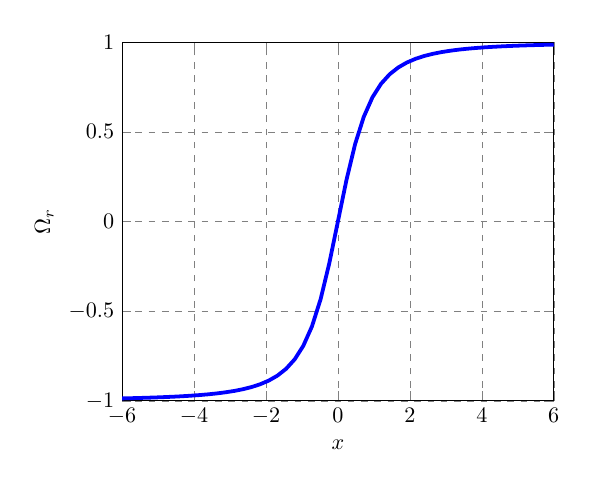
\begin{tikzpicture}[scale=0.8] \begin{axis}[
  xlabel=$x$,
  ylabel=$\Omega_r$,
  grid=major, 
  major grid style={color=gray,line width=0.2pt, dashed},
  xmin=-6, xmax=6,
  ymin=-1, ymax=1 ]
  \addplot[
    domain=-6:6,domain y=-1:1, samples=51, line width=0.6mm, color=blue
  ]
  {x/sqrt( 1 + x*x)};
  \end{axis}
  \end{tikzpicture}
\end{subfigure}
\hspace{2cm}
\begin{subfigure}{5cm}
  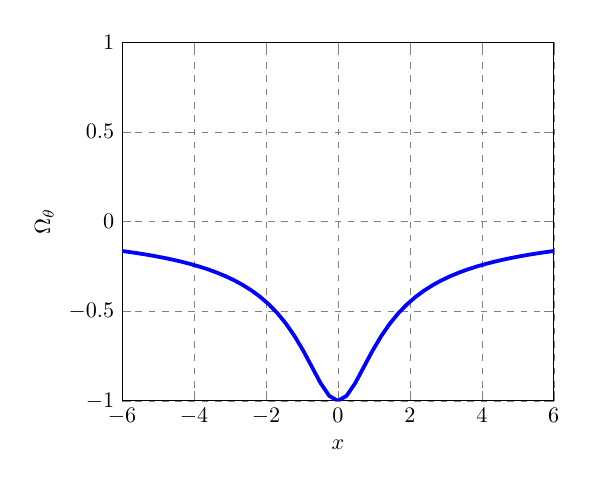
\begin{tikzpicture}[scale=0.8] \begin{axis}[
  xlabel=$x$,
  ylabel=$\Omega_\theta$,
  grid=major, 
  major grid style={color=gray,line width=0.2pt, dashed},
  xmin=-6, xmax=6,
  ymin=-1, ymax=1 ]
  \addplot[
    domain=-6:6,domain y=-1:1, samples=51, line width=0.6mm, color=blue
  ]
  {-1/sqrt( 1 + x*x)};
  \end{axis}
  \end{tikzpicture}
\end{subfigure}
\caption{Vector components of straight line trajectory in $x$ direction along $(x,1)$ in polar coordinates.}
\label{Fig:vector_straightTrajectoryPolarCoordinate_ComponentPlots}
\end{center}
\end{figure}

The components are plotted in Fig.~\ref{Fig:vector_straightTrajectoryPolarCoordinate_ComponentPlots}. Moving from left to right, the radial component $\Omega_r$ starts near $-1$ crosses the origin at $x = 0$ and proceeds to 1, whereas the polar angle component $\Omega_\theta$ is always negative, starting toward zero, reaching a maximum of $-1$ at $x = 0$, and going again toward zero.

\begin{figure}[tb!]
\begin{center}
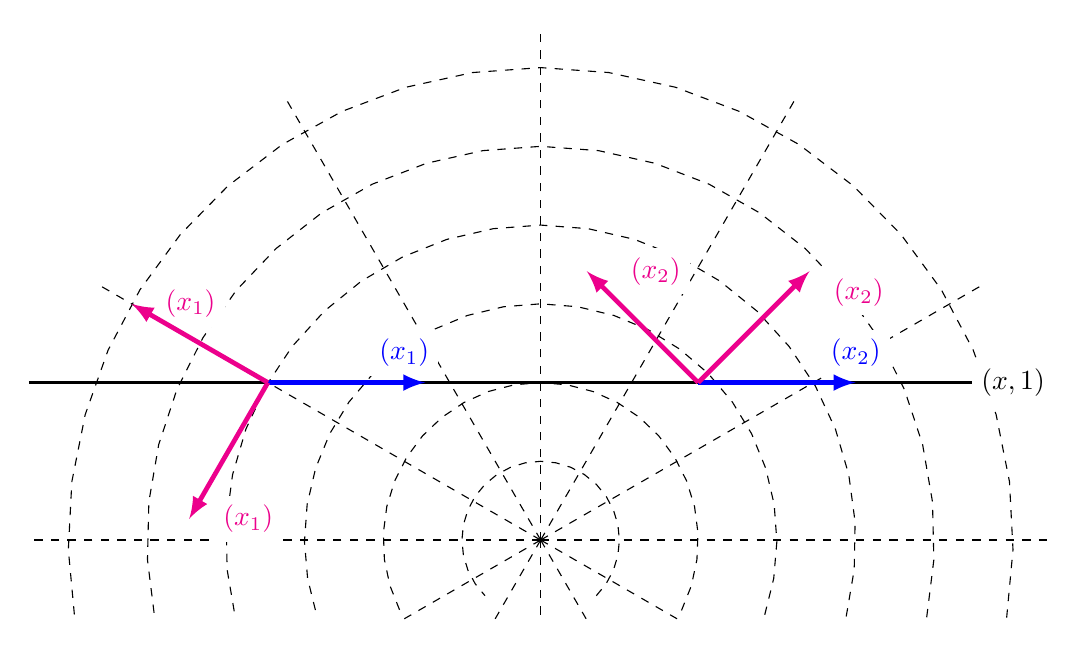
\begin{tikzpicture}
  \foreach \r in {1, 2, 3, 4, 5, 6} 
    \draw[dashed,domain={atan2(-1,\r)}:{360+atan2(-1,-\r)}] plot ({\r*cos(\x)}, {\r*sin(\x)});;
  \foreach \t in {0, 30, 60, 90, 120, 150, 180}
     \draw[dashed] (0,0) -- ({6.5*cos(\t))},{6.5*sin(\t))});
  \foreach \t in {-30, -60, -90, -120, -150}
     \draw[dashed] (0,0) -- ({-cot(\t))},{max(-1,6.5*sin(\t)))});
  
  \node[color=blue,fill=white] at ({2*cos(150)},{4*sin(150) + 0.375}) {$\dir(x_1)$};
  \node[color=magenta,fill=white] at ({0.75 + 6*cos(150)},{6*sin(150)}) {$\rhat(x_1)$};
  \node[color=magenta,fill=white] at ({0.75 + 4*cos(150) + 2*cos(240)},{4*sin(150) + 2*sin(240)}) {$\thetahat(x_1)$};

%  \node[color=blue,fill=white] at ({2+4*sin(150)*cot(60)},{4*sin(150) + 0.375}) {$\dir(x_2)$};
%  \node[color=magenta,fill=white] at ({0.625 + 4*sin(150)*cot(60) + 2*cos(60)},{4*sin(150) + 2*sin(60)}) {$\rhat(x_2)$};
%  \node[color=magenta,fill=white] at ({0.875 + 4*sin(150)*cot(60) + 2*cos(150)},{4*sin(150) + 2*sin(150)}) {$\thetahat(x_2)$};
  \node[color=blue,fill=white] at ({2+4*sin(150)*cot(45)},{4*sin(150) + 0.375}) {$\dir(x_2)$};
  \node[color=magenta,fill=white] at ({0.625 + 4*sin(150)*cot(45) + 2*cos(45)} ,{4*sin(150) + 2*sin(35)}) {$\rhat(x_2)$};
  \node[color=magenta,fill=white] at ({0.875 + 4*sin(150)*cot(45) + 2*cos(135)},{4*sin(150) + 2*sin(135)}) {$\thetahat(x_2)$};


  \draw[line width=0.3mm] (-6.5,{4*sin(150)}) -- (6.5,{4*sin(150)});
  \node[fill=white] at (6,{4*sin(150)}) {$(x,1)$};

  \draw[-latex,color=blue,line width=0.6mm] ({4*cos(150)},{4*sin(150)}) -- +(2,0);
  \draw[-latex,color=magenta,line width=0.6mm] ({4*cos(150)},{4*sin(150)}) -- + ({2*cos(150)},{2*sin(150)});
  \draw[-latex,color=magenta,line width=0.6mm] ({4*cos(150)},{4*sin(150)}) -- + ({2*cos(240)},{2*sin(240)});

%  \draw[-latex,color=blue,line width=0.6mm] ({4*sin(150)*cot(60)},{4*sin(150)}) -- +(2,0);
%  \draw[-latex,color=magenta,line width=0.6mm] ({4*sin(150)*cot(60)},{4*sin(150)}) -- + ({2*cos(60)},{2*sin(60)});
%  \draw[-latex,color=magenta,line width=0.6mm] ({4*sin(150)*cot(60)},{4*sin(150)}) -- + ({2*cos(150)},{2*sin(150)});
  \draw[-latex,color=blue,line width=0.6mm] ({4*sin(150)*cot(45)},{4*sin(150)}) -- +(2,0);
  \draw[-latex,color=magenta,line width=0.6mm] ({4*sin(150)*cot(45)},{4*sin(150)}) -- + ({2*cos(45)},{2*sin(45)});
  \draw[-latex,color=magenta,line width=0.6mm] ({4*sin(150)*cot(45)},{4*sin(150)}) -- + ({2*cos(135)},{2*sin(135)});
\end{tikzpicture}
\caption{Illustration of a couple vector locations for the straight-line trajectory alongside the corresponding basis vectors.}
\label{Fig:vector_straightTrajectoryPolarCoordinate_ExampleVectors}
\end{center}
\end{figure}

To help understand this behavior for $y = 1$, two vectors $\dir$ at different values of $x$ are plotted in Fig.~\ref{Fig:vector_straightTrajectoryPolarCoordinate_ExampleVectors} in blue along with the corresponding basis vectors in magenta. For the negative values of $x$, the cosine of the angle between $\rhat$ and the vector $\dir$ is negative, meaning the radial component of the vector is also negative. When the vector $\dir$ crosses the $y$ axis, it is perpendicular to the $\rhat$ and therefore the radial coordinate is zero. Correspondingly, when $x$ is positive, the cosine of the angle between $\dir$ and $\rhat$ is also positive. As $x$ gets large in either the positive or negative direction, the vector $\dir$ becomes increasingly aligned with $\rhat$.

In terms of $\thetahat$, for negative values of $x$, the dot product is negative. The same is true for positive $x$, as $\thetahat$ is always aligned in a direction that is counterclockwise and tangent to a circle about the origin. Note that as $x$ approaches the origin from the left, the angle between $\dir$ and $\thetahat$ approaches 180$^\circ$. As $x$ moves away from the points $y$ axis, the angle between $\dir$ and $\thetahat$ continues to decrease and tends toward 90$^\circ$. Since the range of the angle between $\dir$ and $\thetahat$ ranges from 270$^\circ$ to 90$^\circ$, the cosine is always negative and $\Omega_\theta$ is always negative. Note that if we send the trajectory for a fixed value of $-y$, then the $\Omega_\theta$ component would always be positive.


%%%%%%%%%%%%%%%%%%%%%%%%%%%%%%%%%%%%%%%%%%%%%%%%%%%%%%%%%%%%%%%%%%%%%%%%%%%%%%%%%%%%%%%%%%%%%%%
\subsection{Gradient in Non-Cartesian Coordinates}

One of the advantages of the vector notation is that it is independent of coordinate system. Thus far, we have discussed how to perform the gradient and its associated operators in Cartesian coordinates. 

Here we show how to obtain the gradient in general coordinates. Suppose we have a coordinate system with coordinate indices $(u,v,w)$ and respective basis vectors $\evec_u$, $\evec_v$, and $\evec_w$. Suppose we express the gradient in terms of the basis vectors with unknown coefficients 
\begin{align}
  \nabla f = A_u \evec_u + A_v \evec_v + A_w \evec_w .
\end{align}
Next we take the directional derivative along each of the directions
\begin{subequations}
\begin{align}
  \dho{f}{u} &= \evec_u \cdot \nabla f = A_u ( \evec_u \cdot \evec_u ) + A_v ( \evec_u \cdot \evec_v ) + A_w ( \evec_u \cdot \evec_w ), \\
  \dho{f}{v} &= \evec_v \cdot \nabla f = A_u ( \evec_v \cdot \evec_u ) + A_v ( \evec_v \cdot \evec_v ) + A_w ( \evec_v \cdot \evec_w ), \\
  \dho{f}{w} &= \evec_w \cdot \nabla f = A_u ( \evec_w \cdot \evec_u ) + A_v ( \evec_w \cdot \evec_v ) + A_w ( \evec_w \cdot \evec_w ) .
\end{align}
\end{subequations}
This can be written as the following linear system:
\begin{align}
  \left[ \begin{array}{c c c} 
  \evec_u \cdot \evec_u & \evec_u \cdot \evec_v & \evec_u \cdot \evec_w \\
  \evec_v \cdot \evec_u & \evec_v \cdot \evec_v & \evec_v \cdot \evec_w \\
  \evec_w \cdot \evec_u & \evec_w \cdot \evec_v & \evec_w \cdot \evec_w \\ \end{array} \right]
  \left[ \begin{array}{c} A_u \\ A_v \\ A_w \\ \end{array} \right] = 
  \left[ \begin{array}{c} \dho{f}{u} \vspace{0.2cm} \\  \dho{f}{v} \vspace{0.2cm} \\ \dho{f}{w} \\ \end{array} \right]
\end{align}
Recall that this matrix is the metric tensor $\mathbf{g}$ from linear algebra. To compute the elements of the metric tensor, we express the basis vectors in terms of Cartesian coordinate partial derivatives using the multivariable chain rule. For example:
\begin{align}
  \evec_u \cdot \evec_v &= \left( \dho{x}{u} \evec_x + \dho{y}{u} \evec_y + \dho{z}{u} \evec_z \right) \cdot \left( \dho{x}{v} \evec_x + \dho{y}{v} \evec_y + \dho{z}{v} \evec_z \right) \nonumber \\
  &= \dho{x}{u} \dho{x}{v} + \dho{y}{u} \dho{y}{v} + \dho{z}{u} \dho{z}{v} .
\end{align}
The cross terms vanish because $\evec_x \cdot \evec_y = 0$, $\evec_x \cdot \evec_z = 0$, and $\evec_y \cdot \evec_z = 0$. Once these products of partial derivatives have been computed, we can find each element of the metric tensor and solve the linear system of equations by finding the inverse metric tensor $\mathbf{g}^{-1}$ to obtain the coefficients.


%%%%%%%%%%%%%%%%%%%%%%%%%%%%%%%%%%%%%%%%%%%%%%%%%%%%%%%%%%%%%%%%%%%%%%%%%%%%%%%%%%%%%%%%%%%%%%%
\subsection{Example: Gradient in Spherical Coordinates}

To illustrate this, let us compute the gradient in spherical coordinates. Recall that
\begin{align}
  x &= r \sin \theta \cos \phi , \nonumber \\
  y &= r \sin \theta \sin \phi, \nonumber  \\
  z &= r \cos \theta . \nonumber 
\end{align}
Taking the partial derivatives and evaluating the products of basis vectors
\begin{subequations}
\begin{align}
  \evec_r \cdot \evec_r      &= \sin^2 \theta \cos^2 \phi + \sin^2 \theta \sin^2 \phi + \cos^2 \theta = 1, \\
  \evec_r \cdot \evec_\theta &= r \sin \theta \cos \theta \cos^2 \phi + r \cos \theta \cos \theta \sin^2 \phi - r \cos \theta \sin \theta  = 0, \\
  \evec_r \cdot \evec_\phi   &= - r \sin^2 \theta \sin \phi \cos \phi + r \sin^2 \theta \sin \phi \cos \phi = 0, \\
  \evec_\theta \cdot \evec_\theta &= r^2 \cos^2 \theta \cos^2 \phi + r^2 \cos^2 \theta \sin^2 \phi + r^2 \sin^2 \theta = r^2, \\
  \evec_\theta \cdot \evec_\phi   &= -r^2 \sin \theta \cos \theta \sin \phi \cos \phi + r^2 \sin \theta \cos \theta \sin \phi \cos \phi = 0, \\
  \evec_\phi \cdot \evec_\phi     &= r^2 \sin^2 \theta \sin^2 \phi + r^2 \sin^2 \theta \cos^2 \phi = r^2 \sin^2 \theta .
\end{align}
\end{subequations}
Note that the cross terms are all zero; this is a consequence of the spherical coordinate system being orthogonal. The linear system with the metric tensor becomes:
\begin{align}
  \left[ \begin{array}{c c c} 
  1 & 0   & 0 \\
  0 & r^2 & 0 \\
  0 & 0   & r^2 \sin^2 \theta \\ \end{array} \right]
  \left[ \begin{array}{c} A_r \\ A_\theta \\ A_\phi \\ \end{array} \right] = 
  \left[ \begin{array}{c} \dho{f}{r} \vspace{0.2cm} \\  \dho{f}{\theta} \vspace{0.2cm} \\ \dho{f}{\phi} \\ \end{array} \right] .
\end{align}
Since the metric tensor for this coordinate system is diagonal, we can easily invert to solve the system:
\begin{align}
  \left[ \begin{array}{c} A_r \\ A_\theta \\ A_\phi \\ \end{array} \right] = 
  \left[ \begin{array}{c c c} 
  1 & 0   & 0 \vspace{0.2cm}  \\
  0 & \dfrac{1}{r^2} & 0 \vspace{0.2cm} \\
  0 & 0   & \dfrac{1}{r^2 \sin^2 \theta} \vspace{0.2cm} \\ \end{array} \right]
  \left[ \begin{array}{c} \dho{f}{r} \vspace{0.2cm} \\  \dho{f}{\theta} \vspace{0.2cm} \\ \dho{f}{\phi} \\ \end{array} \right] .
\end{align}
Therefore, the gradient is
\begin{align}
  \nabla f = \dho{f}{r} \evec_r + \frac{1}{r^2} \dho{f}{\theta} \evec_\theta + \frac{1}{r^2 \sin^2 \theta} \dho{f}{\phi} \evec_\phi .
\end{align}
We generally express the gradient in terms of the unit basis vectors to make the coordinate system orthonormal. The gradient with the orthonormal spherical basis vectors is
\begin{align}
  \nabla f = \dho{f}{r} \rhat + \frac{1}{r} \dho{f}{\theta} \thetahat + \frac{1}{r \sin \theta} \dho{f}{\phi} \phihat .
\end{align}


%%%%%%%%%%%%%%%%%%%%%%%%%%%%%%%%%%%%%%%%%%%%%%%%%%%%%%%%%%%%%%%%%%%%%%%%%%%%%%%%%%%%%%%%%%%%%%%
\subsection{Metric Tensor and Scale Factors}

In the derivation for the gradient, we found the metric tensor,
\begin{align}
  \mathbf{g} = \left[ \begin{array}{c c c} 
  \evec_u \cdot \evec_u & \evec_u \cdot \evec_v & \evec_u \cdot \evec_w \\
  \evec_v \cdot \evec_u & \evec_v \cdot \evec_v & \evec_v \cdot \evec_w \\
  \evec_w \cdot \evec_u & \evec_w \cdot \evec_v & \evec_w \cdot \evec_w \\ \end{array} \right] ,
\end{align}
arise. Recall from linear algebra (where the basis vectors are constant everywhere) the metric tensor is used to measure distance and angles between vectors. In the context of calculus, where we allow the basis vectors to change continuously with position, the metric tensor takes on the meaning that allows us to consistently measure differential length in each coordinate direction at each point in space.

The curvilinear coordinate systems all have the property of orthogonality, which means that the basis vectors are orthogonal at all points in space. When this occurs, the off-diagonal terms of the metric tensor goes to zero, as we saw for spherical coordinates. Therefore, for orthogonal coordinate systems, we can write the metric tensor as
\begin{align}
  \mathbf{g} = \left[ \begin{array}{c c c} 
  \evec_u \cdot \evec_u & 0                     & 0                     \\
                      0 & \evec_v \cdot \evec_v & 0                     \\
                      0 &                     0 & \evec_w \cdot \evec_w \\ \end{array} \right]
  = \left[ \begin{array}{c c c} 
  h_u^2 &     0 &     0  \\
      0 & h_v^2 &     0 \\
      0 &     0 & h_w^2 \\ \end{array} \right] .
\end{align}
Here the $h$ factors are called the \emph{scale factors}, which are the square root of the diagonal elements of the metric tensor in an orthogonal coordinate system: 
\begin{align}
  h_i = \sqrt{ g_{ii} } .
\end{align}
The scale factors allow us to develop general formulas for the gradient, divergence, and curl. They also permit us to put the coordinate systems into an orthonormal form having unit basis vectors. Note that it is important to emphasize that this only applies in orthogonal coordinate systems. Fortunately, non-orthogonal curvilinear coordinates (called skew coordinates) are seldom used in scientific and engineering applications, so knowing the forms for orthogonal coordinate systems is almost always sufficient.

The scale factors for Cartesian coordinates are:
\begin{subequations}
\begin{align}
  h_x &= 1, \\
  h_y &= 1, \\
  h_z &= 1. 
\end{align}
\end{subequations}
The scale factors for cylindrical coordinates are
\begin{subequations}
\begin{align}
  h_r &= 1, \\
  h_\theta &= r, \\
  h_z &= 1. 
\end{align}
\end{subequations}
Finally, the scale factors for spherical coordinates are
\begin{subequations}
\begin{align}
  h_r &= 1, \\
  h_\theta &= r, \\
  h_\phi &= r \sin \theta. 
\end{align}
\end{subequations}


%%%%%%%%%%%%%%%%%%%%%%%%%%%%%%%%%%%%%%%%%%%%%%%%%%%%%%%%%%%%%%%%%%%%%%%%%%%%%%%%%%%%%%%%%%%%%%%
\subsection{Gradient, Divergence, and Curl in Curvilinear Coordinates}

Using the scale factors, we can develop expressions for the gradient, divergence, curl, and Laplacian that apply to any orthonormal coordinate system. The gradient is
\begin{align}
  \nabla f = \frac{1}{h_u} \dho{f}{u} \hat{\mathbf{u}} + \frac{1}{h_v} \dho{f}{v} \hat{\mathbf{v}} + \frac{1}{h_w} \dho{f}{w} \hat{\mathbf{w}},
\end{align}
where $\hat{\mathbf{u}}$, $\hat{\mathbf{v}}$, and $\hat{\mathbf{w}}$ are normalized unit basis vectors. The divergence is
\begin{align}
  \nabla \cdot \mathbf{F} &= \frac{1}{h_u h_v h_w} \left[ \dho{}{u}( h_v h_w F_u ) +  \dho{}{v}( h_u h_w F_v ) + \dho{}{w} ( h_u h_v F_w ) \right] .
\end{align}
The curl is given by
\begin{align}
  \nabla \times \mathbf{F} &= \frac{1}{h_u h_v h_w}
  \left| \begin{array}{c c c}
  h_u \uhat & h_v \vhat & h_w \what \vspace{0.2cm} \\
  \dfrac{\partial}{\partial u} & \dfrac{\partial}{\partial v} & \dfrac{\partial}{\partial w} \vspace{0.2cm}  \\
  h_u F_u   & h_v F_v   & h_w F_w   \\ \end{array} \right| .
\end{align}
The scalar Laplacian is
\begin{align}
  \nabla^2 f = \frac{1}{h_u h_v h_w} 
    \left[ \dho{}{u} \left( \frac{h_v h_w}{h_u} \dho{f}{u} \right) 
         + \dho{}{v} \left( \frac{h_u h_w}{h_v} \dho{f}{v} \right) 
         + \dho{}{w} \left( \frac{h_u h_v}{h_w} \dho{f}{w} \right) \right] .
\end{align}

Applying these to cylindrical coordinates, we obtain the following expressions for the gradient, divergence, curl, and Laplician:
\begin{subequations}
\begin{align}
  \nabla f &= \dho{f}{r} \rhat + \frac{1}{r} \dho{f}{\theta} \thetahat + \dho{f}{z} \zhat , \\
  \nabla \cdot \mathbf{F} &= \frac{1}{r} \dho{}{r}(r F_r) + \frac{1}{r} \dho{F_\theta}{\theta} + \dho{F_z}{z} , \\
  \nabla \times \mathbf{F} &= 
    \frac{1}{r} \left( \dho{F_z}{\theta} - \dho{}{z} ( r F_\theta ) \right) \rhat 
  +             \left( \dho{F_r}{z} - \dho{F_z}{r}  \right) \thetahat \nonumber \\
  &+ \frac{1}{r} \left(  \dho{}{r} ( r F_\theta ) - \dho{F_r}{\theta} \right) \zhat , \\
  \nabla^2 f &= \frac{1}{r} \dho{}{r} \left( r \dho{f}{r} \right) + \frac{1}{r^2} \dhotwo{f}{\theta} + \dhotwo{f}{z} .
\end{align}
\end{subequations}
The gradient, divergence, curl, and Laplician in spherical coordinates are:
\begin{subequations}
\begin{align}
  \nabla f &=   \dho{f}{r} \rhat + \frac{1}{r} \dho{f}{\theta} \thetahat + \frac{1}{r \sin \theta} \dho{f}{\phi} \phihat , \\
  \nabla \cdot \mathbf{F} &= \frac{1}{r^2} \dho{}{r} ( r^2 F_r ) + \frac{1}{r \sin \theta} \dho{}{\theta} ( \sin \theta F_\theta ) + \frac{1}{r \sin \theta} \dho{F_\phi}{\phi}, \\
  \nabla \times \mathbf{F} &= 
    \frac{1}{r \sin \theta} \left( \dho{}{\theta} ( \sin \theta F_\phi ) - \dho{F_\theta}{\phi} \right) \rhat
  + \frac{1}{r} \left( \frac{1}{\sin \theta } \dho{F_r}{\phi} -  \dho{}{r} ( r F_\phi ) \right) \thetahat \nonumber \\
 &+ \frac{1}{r} \left( \dho{}{r} ( r F_\theta ) - \dho{ F_r }{ \theta } \right) \phihat , \\
   \nabla^2 f &= \frac{1}{r^2} \dho{}{r} \left( r^2 \dho{f}{r} \right) 
               + \frac{1}{r^2 \sin \theta } \dho{}{\theta} \left( \sin \theta \dho{f}{\theta} \right) 
               + \frac{1}{r^2 \sin^2 \theta } \dhotwo{f}{\phi} .
\end{align}
\end{subequations}


%%%%%%%%%%%%%%%%%%%%%%%%%%%%%%%%%%%%%%%%%%%%%%%%%%%%%%%%%%%%%%%%%%%%%%%%%%%%%%%%%%%%%%%%%%%%%%%
%%%%%%%%%%%%%%%%%%%%%%%%%%%%%%%%%%%%%%%%%%%%%%%%%%%%%%%%%%%%%%%%%%%%%%%%%%%%%%%%%%%%%%%%%%%%%%%
\section{Covector Fields}

The gradient operator takes a scalar field and converts it into a vector field. Recall for linear algebra that column vectors are vectors, whereas row vectors are covectors. It is therefore reasonable to ask whether there is an analogous covector field. The answer is yes, and it is related to the differential of a scalar field $df$. To understand that the differential operator takes a vector field and produces a covector field, we must define the differential or ``$d$'' operator in a specific way. Given this new interpretation of the differential $df$, we can develop a connection for line integration to linear algebra.

%%%%%%%%%%%%%%%%%%%%%%%%%%%%%%%%%%%%%%%%%%%%%%%%%%%%%%%%%%%%%%%%%%%%%%%%%%%%%%%%%%%%%%%%%%%%%%%
\subsection{Directional Derivative and the Differential Operator}

Traditionally we think of $dx$ as a small change in the variable $x$. Consider the consider simple the scalar field $f = x$. This scalar field simply takes on the $x$ value at each point. Now suppose we take the directional derivative along the $\mathbf{v}$ direction of this scalar field that we equate to some $dx$ operating upon $\mathbf{v}$:
\begin{align}
  dx( \mathbf{v} ) = \nabla_{\mathbf{v}} x = \mathbf{v} \cdot \nabla x = \mathbf{v} \cdot \evec_x = v_x,
\end{align}
which is simply the $x$ component of the vector $\mathbf{v}$. We may think of the operator $dx$ as taking the $x$ component of some vector. An equivalent formulation is to write $dx$ as a row vector
\begin{align}
  dx = \left[ \begin{array}{c c c} 1 & 0 & 0 \\ \end{array} \right] = \epsilon_x,
\end{align}
which is equivalent to the Cartesian basis covector $\epsilon_x$. Recall that the basis covector is a set of vertical parallel lines (in 2-D space) or planes (in 3-D space) oriented in the $x$ direction. Likewise, $dy = \epsilon_y$ and $dz = \epsilon_z$ which are lines or planes with the respective $y$ and $z$ orientations.

We can now take the differential of a scalar field $f$ by applying the multivariable chain rule:
\begin{align}
  df = \dho{f}{x} dx + \dho{f}{y} dy + \dho{f}{z} dz .
\end{align}
This says that the differential change in $f$ is equal to the differential change in $x$ times the partial derivative of $f$ with respect to $x$, plus the differential change in $y$ times the partial derivative of $f$ with respect to $y$, and similarly for $z$. In the context of the directional derivative $df$ acting on vector $\mathbf{v}$ gives the instantaneous rate of change of $f$ along $\mathbf{v}$. From the multivariable chain rule, this can be written as the sum of Cartesian basis covector fields.

\begin{figure}[!tb]
\begin{center}
\begin{subfigure}[b]{0.3\textwidth}
  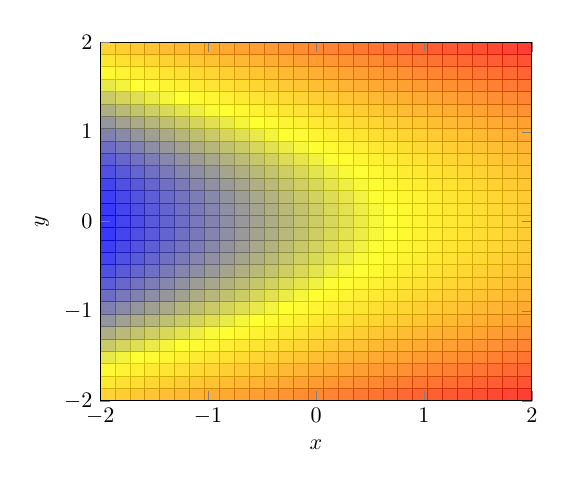
\begin{tikzpicture}[scale=0.8] \begin{axis}[xlabel=$x$,ylabel=$y$,view={0}{90}]
  \addplot3[
    surf,
    opacity=0.8,
    samples=30, samples y=30,
    domain=-2:2,domain y=-2:2
  ]
  {x + y*y - 1};
  \end{axis}
  \end{tikzpicture}
\end{subfigure}
\hspace{2cm}
\begin{subfigure}[b]{0.3\textwidth}
  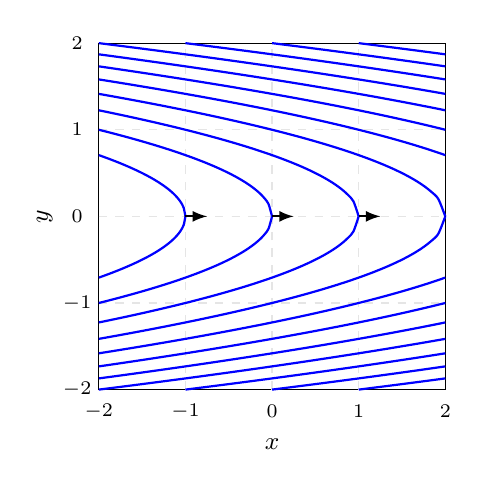
\begin{tikzpicture}[scale=1.1]
  \draw (-2,-2) -- (2,-2) -- (2,2) -- (-2,2) -- cycle;
  \node at (0,-2.625) {\small $x$};
  \node[rotate=90] at (-2.625,0) {\small $y$};
  \foreach \x in {-1,0,1} 
      \foreach \y in {-1,0,1} 
        { 
          \draw[dashed,color=gray!20] (\x,-2) -- (\x,2);
          \draw[dashed,color=gray!20] (-2,\y) -- (2,\y);
        } 


  \foreach \x in {-2,-1,0,1,2}
     \node at (\x,-2.25) {\scriptsize $\x$};
  \foreach \y in {-2,-1,0,1,2} 
      \node at (-2.25,\y) {\scriptsize $\y$};

  \foreach \r in {-1,...,9} {
    \draw[thick,color=blue]   plot[smooth,domain={max(-2,-\r)}:{min(2,8-\r)},samples=51] ({-\x}, { sqrt(0.5*\r + 0.5*\x)});
    \draw[thick,color=blue]   plot[smooth,domain={max(-2,-\r)}:{min(2,8-\r)},samples=51] ({-\x}, {-sqrt(0.5*\r + 0.5*\x)});
  }
  
  \foreach \x in {-1,0,1} {
    \draw[-latex,thick] (\x,0) -- +(0.25,0);
  }
  
  \end{tikzpicture}

\end{subfigure}

\caption{Depiction of a scalar field $f(x,y) = x + y^2 - 1$ and its associated covector field $df = dx + 2y dy$.}
\label{Fig:vector_covectorFieldExample}
\end{center}
\end{figure}


To illustrate this geometrically, consider the 2-D scalar field 
\begin{align}
  f(x,y) = x + y^2 - 1. 
\end{align}
The differential operator acting upon $f$ gives
\begin{align}
  df = dx + 2y dy. 
\end{align}
Writing these as covectors:
\begin{align}
  df = \left[ \begin{array}{c c} 1 & 0 \\ \end{array} \right] + 2 y \left[ \begin{array}{c c} 0 & 1 \\ \end{array} \right]  = \left[ \begin{array}{c c} 1 & 2y \\ \end{array} \right].
\end{align}
As we saw in linear algebra, the covectors can be thought of as lines of constant ``elevation''. Let us suppose $df$ now acts on some position vector $\mathbf{R} = x \evec_x + y \evec_y$:
\begin{align}
  df(\mathbf{R}) = \left[ \begin{array}{c c} 1 & 2y \\ \end{array} \right]
  \left[ \begin{array}{c} x \\ y \\ \end{array} \right] = x + 2y^2 = r.
\end{align}
Here $r$ represents some scalar number. Represented graphically, a fixed value of $r$ gives a curve. (Recall in linear algebra, since things were not functions of space, the curves were simple lines). Several such curves are plotted in Fig.~\ref{Fig:vector_covectorFieldExample} along with the associated scalar field. These curves can be thought of as contour lines of the scalar field. The density of these lines along a direction gives a measure of how much the scalar field is changing along that direction, which is similar to lines of constant elevation of a terrain map.

To be more precise, the differential operator $d$ acting upon $f$ maps a scalar field to a covector field, which is analogous to how the gradient operator $\nabla$ acting upon $f$ maps a scalar field maps to a vector field. As with vector fields, a covector field assigns a covector to every point in space. To compute the directional derivative with respect to a constant vector $\mathbf{v}$ at some point $(x,y)$ we evaluate the covector field and get a stack of parallel lines (or parallel planes in 3-D space) and then make a count (in a continuous sense) of the number of lines that vector $\mathbf{v}$ pierces.

\begin{figure}[!tb]
\begin{center}
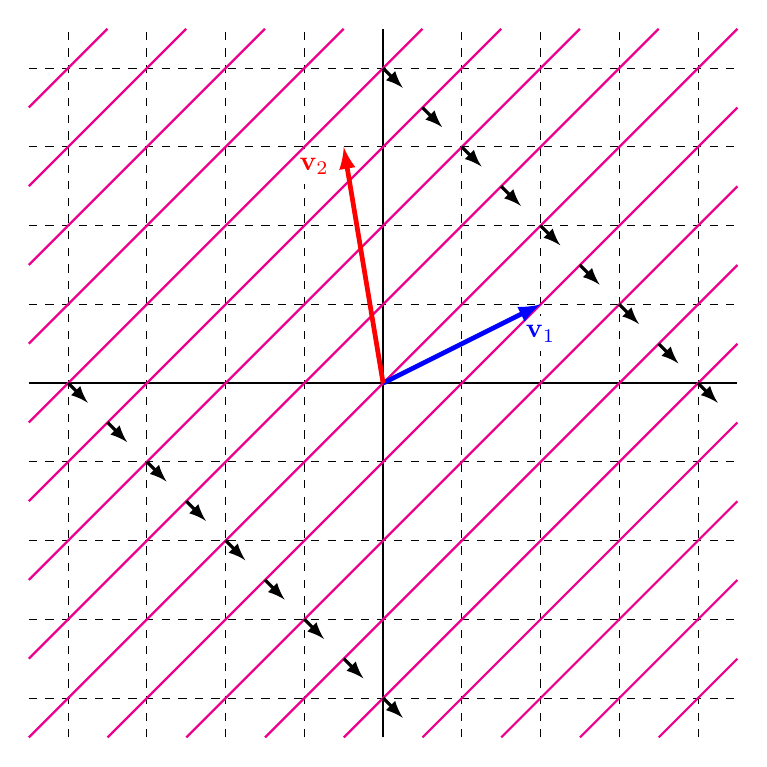
\begin{tikzpicture}
  \draw[thick] (-4.5,0) -- (4.5,0);
  \draw[thick] (0,-4.5) -- (0,4.5);
  \foreach \x in {-4,...,4}
    \draw[dashed] (\x,-4.5) -- (\x,4.5);
  \foreach \y in {-4,...,4}
    \draw[dashed] (-4.5,\y) -- (4.5,\y);
    
  \node[color=blue,fill=white] at (2,0.625) {$\mathbf{v}_1$};  
  \node[color=red,fill=white] at (-0.875,2.75)  {$\mathbf{v}_2$};  
    
  \foreach \r in {-8,...,8} {
    \draw[thick,color=magenta] ({max(-4.5,-4.5 + \r},{max(-4.5,-4.5-\r)}) -- ({min(4.5,4.5 + \r)},{min(4.5,4.5 - \r)});
  }
  \foreach \r in {-4,...,4} {
    \draw[-latex,line width=0.4mm] ({2 + 0.5*\r},{2 - 0.5*\r}) -- +(0.25,-0.25);
  }
  \foreach \r in {-4,...,4} {
    \draw[-latex,line width=0.4mm] ({-2 + 0.5*\r},{-2 - 0.5*\r}) -- +(0.25,-0.25);
  }
  
  \draw[-latex,line width=0.6mm,color=blue] (0,0) -- (2,1);
  \draw[-latex,line width=0.6mm,color=red]  (0,0) -- (-0.5,3);
\end{tikzpicture}

\caption{Depiction of the directional derivative using the covector field $df = dx + 2y dy$ evaluated at $(1,-\rfrac{1}{2})$ with a vectors $\mathbf{v}_1 = 2 \evec_x + \evec_y$ and $\mathbf{v}_2 = -\rfrac{1}{2} \evec_x + 3 \evec_y$.}
\label{Fig:vector_covectorFieldExample_atPoint}
\end{center}
\end{figure}

Returning to the example, if we wish to evaluate the directional derivative at point $(1,-\rfrac{1}{2})$, we evaluate the covector field at that point
\begin{align}
  df = \left[ \begin{array}{c c} 1 & -1 \\ \end{array} \right] . \nonumber
\end{align}
Suppose now this covector acts upon a vector $\mathbf{v}_1 = 2 \evec_x + \evec_y$. This gives
\begin{align}
  df( \mathbf{v}_1 ) = \left[ \begin{array}{c c} 1 & -1 \\ \end{array} \right] 
  \left[ \begin{array}{c} 2 \\ 1 \\ \end{array} \right] = 1. \nonumber
\end{align}
This is illustrated graphically in Fig.~\ref{Fig:vector_covectorFieldExample_atPoint}. The vector $\mathbf{v}_1$ pierces one covector line in the positive direction and therefore the directional derivative of $\mathbf{v}_1$ at the point $(1,-\rfrac{1}{2})$ point is 1. The sign is positive since the vector is moving along with the direction indicated by the covector planes (this could be thought of as increasing elevation).

We can also take the directional derivative along $\mathbf{v}_2 = -\rfrac{1}{2} \evec_x + 3 \evec_y$ at $(1,-\rfrac{1}{2})$. The result of this multiplication gives
\begin{align}
  df( \mathbf{v}_2 ) = \left[ \begin{array}{c c} 1 & -1 \\ \end{array} \right] 
  \left[ \begin{array}{c} -\rfrac{1}{2} \\ 3 \\ \end{array} \right] = -\frac{7}{2}. \nonumber
\end{align}
This is because the vector goes through 3.5 covector lines, but in the direction of decreasing contour lines.

The covector field is often referred to as a differential form, or more precisely a differential 1-form. The concept of a 1-form is used to define integration along a curved path, where each differential unit of length traversed along the path is multiplied by the covector field or 1-form at that path. While we will not go into this in these notes, we can also write 2-forms and 3-forms, which are used to define surface and volume integrals.


%%%%%%%%%%%%%%%%%%%%%%%%%%%%%%%%%%%%%%%%%%%%%%%%%%%%%%%%%%%%%%%%%%%%%%%%%%%%%%%%%%%%%%%%%%%%%%%
%%%%%%%%%%%%%%%%%%%%%%%%%%%%%%%%%%%%%%%%%%%%%%%%%%%%%%%%%%%%%%%%%%%%%%%%%%%%%%%%%%%%%%%%%%%%%%%
\section{Line Integrals}

Some problems in physics and engineering involve evaluating integrals of functions along trajectories. Herein we refer to the idea as taking a line integral and the trajectory is given by path $P(a,b)$ with endpoints given by locations $a$ and $b$ along the path. We may then take the integral of some scalar field $f(x,y,z)$. It is common to parameterize the path with some common variable $t$ such that the variables $(x,y,z)$ can be written in terms of the parameter $t$, which we often take to be time. The integrals in terms of that parameter $t$ can be written as
\begin{align}
  \int_{P(a,b)} f(t) dt .
\end{align}

In many applications (e.g., finding the work done by a force field) we take the line integral with respect to a vector field, which is given as
\begin{align}
  \int_{P(a,b)} \mathbf{F} \cdot d\boldsymbol\ell .
\end{align}
Here $d\boldsymbol\ell$ is the differential line vector, which is discussed in the subsequent section.

It is also conventional to take integrals over closed paths, i.e., those that start and end at the same point. For these cases, we denote this with a circle in the integral as such
\begin{align}
  \oint_P \mathbf{F} \cdot d\boldsymbol\ell .
\end{align}


%%%%%%%%%%%%%%%%%%%%%%%%%%%%%%%%%%%%%%%%%%%%%%%%%%%%%%%%%%%%%%%%%%%%%%%%%%%%%%%%%%%%%%%%%%%%%%%
\subsection{Differential Line Vector and Length}

The differential line vector for a general orthogonormal coordinate system $(u,v,w)$ in terms of the scale factors is given by
\begin{align}
  d\boldsymbol\ell =   h_u du \uhat + h_v dv \vhat + h_w dw \what.
\end{align}
Inserting the scale factors for Cartesian, cylindrical, and spherical coordinates gives
\begin{subequations}
\begin{align}
  d\boldsymbol\ell &= dx \ihat + dy \jhat + dz \khat , \\
  d\boldsymbol\ell &= dr \rhat + r d\theta \thetahat + dz \zhat , \\
  d\boldsymbol\ell &= dr \rhat + r d\theta \thetahat + r \sin \theta d\phi \phihat .
\end{align}
\end{subequations}

The differential-length squared for a general orthogonal coordinate system $(u,v,w)$ in terms of the scale factors is given by the dot product of the differential line vector with itself
\begin{align}
  ( d\ell )^2 = d\boldsymbol\ell \cdot d\boldsymbol\ell = ( h_u du )^2 + ( h_v dv )^2 + ( h_w dw )^2 .
\end{align}
Inserting the scale factors for Cartesian, cylindrical, and spherical coordinates gives
\begin{subequations}
\begin{align}
  ( d\ell )^2 &= ( dx )^2 + ( dy )^2 + ( dz )^2, \\
  ( d\ell )^2 &= ( dr )^2 + r^2 ( d\theta )^2 + ( dz )^2, \\
  ( d\ell )^2 &= ( dr )^2 + r^2 ( d\theta )^2 + r^2 \sin^2 \theta ( d\phi )^2 .
\end{align}
\end{subequations}
The differential unit of length $d\ell$ is therefore the square root of $(d\ell)^2$.


%%%%%%%%%%%%%%%%%%%%%%%%%%%%%%%%%%%%%%%%%%%%%%%%%%%%%%%%%%%%%%%%%%%%%%%%%%%%%%%%%%%%%%%%%%%%%%%
\subsection{Example: Moment of Inertia of a Circular Arc}

Suppose we have a wire of fixed radius $R$ constant density $\rho$ shaped into a circular arc. The orientation of the wire is given in Fig.~\ref{Fig:vector_momentOfInertiaCircularArc}. The wire is oriented such that the wire starts at an angle $\theta$ with respect to the $x$-axis and ends at an angle $\phi$ as shown.

\begin{figure}[tb!]
\begin{center}
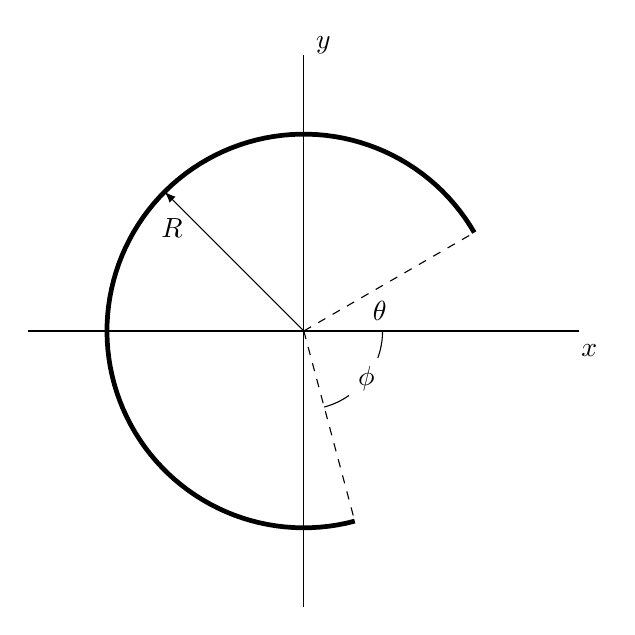
\begin{tikzpicture}
  \draw (-3.5,0) -- (3.5,0);
  \node at (3.625,-0.25) {$x$};
  \draw (0,-3.5) -- (0,3.5);
  \node at (0.25,3.625) {$y$};
  \draw[line width=0.6mm,domain=30:285,samples=101] plot ({2.5*cos(\x)}, {2.5*sin(\x)});
  \draw[dashed] (0,0) -- ({2.5*cos(30)},{2.5*sin(30)});
  \draw[dashed] (0,0) -- ({2.5*cos(285)},{2.5*sin(285)});
  \node at ({1*cos(15)},{1*sin(15)}) {$\theta$};
  \node at ({1*cos(-37.5)},{1*sin(-37.5)}) {$\phi$};
  \draw[domain=-20:0,samples=51] plot ({1*cos(\x)}, {1*sin(\x)});
  \draw[domain=-75:-55,samples=51] plot ({1*cos(\x)}, {1*sin(\x)});
  \draw[-latex] (0,0) -- ({2.5*cos(135)},{2.5*sin(135)});
  \node at ({2.125*cos(142)},{2.125*sin(142)}) {$R$};
\end{tikzpicture}
\caption{Illustration of a circular arc wire.}
\label{Fig:vector_momentOfInertiaCircularArc}
\end{center}
\end{figure}

The moment of inertia describes the resistance of an object to rotation about a specific axis. Using the Cartesian axes, the moments of inertia are given by
\begin{subequations}
\begin{align}
  I_x = \int_{P(a,b)} ( y^2 + z^2 ) \rho(x,y,z) dt, \\
  I_y = \int_{P(a,b)} ( x^2 + z^2 ) \rho(x,y,z) dt, \\
  I_z = \int_{P(a,b)} ( x^2 + y^2 ) \rho(x,y,z) dt .
\end{align}
\end{subequations}
We may parameterize the circular arc as follows:
\begin{subequations}
\begin{align}
  x &= R \cos(t), \\*
  y &= R \sin(t), \\*
  z &= 0,
\end{align}
\end{subequations}
where the parameter $t$ ranges from $\theta$ to $2\pi - \phi$.  Inserting the parameterization into the moment of inertia equations and carrying out the integration gives
\begin{subequations}
\begin{align}
  I_x &= \rho R^2 \int_\theta^{2\pi - \phi} \sin^2(t) dt = \frac{\rho R^2}{2} \left[ 2\pi - \theta - \phi + \frac{1}{2} \left( \sin(2\theta) + \sin(2\phi) \right) \right], \\
  I_y &= \rho R^2 \int_\theta^{2\pi - \phi} \cos^2(t) dt = \frac{\rho R^2}{2} \left[ 2\pi - \theta - \phi - \frac{1}{2} \left( \sin(2\theta) + \sin(2\phi) \right) \right], \\
  I_z &= \rho R^2 \int_\theta^{2\pi - \phi} dt = \rho R^2 ( 2 \pi - \phi - \theta ).
\end{align}
\end{subequations}

%%%%%%%%%%%%%%%%%%%%%%%%%%%%%%%%%%%%%%%%%%%%%%%%%%%%%%%%%%%%%%%%%%%%%%%%%%%%%%%%%%%%%%%%%%%%%%%
\subsection{Example: Work on a Charged Particle by an Electric Field}

Suppose we have a point charged particle (e.g., an electron) with charge $q$ moving in a straight trajectory. The charged particle is in the presence of an electric field generated by a stationary point charge $Q$ at the origin. Coulomb's law for electrostatic point charges in spherical coordinates relates the 
\begin{align}
  \mathbf{F} = \frac{1}{4 \pi \epsilon_0} \frac{qQ}{r^2} \rhat,
\end{align}
where $r$ is the distance between the two point charges and $\epsilon_0$ is a constant called the electric permittivity of free space. The work done by a force is given by
\begin{align}
  W = \int_{P[a,b]} \mathbf{F} \cdot d\boldsymbol\ell .
\end{align}
The most natural coordinate system to use in this case is the spherical coordinate system, for which
\begin{align}
  d\boldsymbol\ell &= dr \rhat + r d\theta \thetahat + r \sin \theta d\phi \phihat . \nonumber
\end{align}
Taking the dot product gives the work as
\begin{align}
   W = \frac{qQ}{4 \pi \epsilon_0} \int_{P[a,b]} \frac{dr}{r^2} .
\end{align}

Since the problem is spherically symmetric, we are free to orient the coordinate system as we wish. The particle moves in a straight-line trajectory, and we can take this to be the $z$ direction with $x$ and $y$ fixed. The trajectory starts at some location $z = a$ and moves to $z = b$. In spherical coordinates
\begin{align}
  r = \sqrt{ x^2 + y^2 + z^2 } . \nonumber
\end{align}
Differentiating with respect to $z$
\begin{align}
  dr = \frac{z}{\sqrt{ x^2 + y^2 + z^2 }} dz .
\end{align}
Inserting this into the equation for work gives
\begin{align}
   W = \frac{qQ}{4 \pi \epsilon_0} \int_a^b \frac{z}{(x^2 + y^2 + z^2)^{3/2}} dz.
\end{align}
Evaluating the integral gives
\begin{align}
   W = \frac{qQ}{4 \pi \epsilon_0} \left[ \frac{1}{\sqrt{x^2 + y^2 + a^2}} - \frac{1}{\sqrt{x^2 + y^2 + b^2}} \right].
\end{align}


%%%%%%%%%%%%%%%%%%%%%%%%%%%%%%%%%%%%%%%%%%%%%%%%%%%%%%%%%%%%%%%%%%%%%%%%%%%%%%%%%%%%%%%%%%%%%%%
\subsection{Example: Circumference of an Ellipse}

To find the circumference of an ellipse, we derive an equation for the arc length. The differential length squared in Cartesian coordinates is
\begin{align}
  ( d\ell )^2 = (dx)^2 + (dy)^2.
\end{align}
We may apply the chain rule to $dx$ and $dy$ to put in terms of some parameter $t$:
\begin{align}
  ( d\ell )^2 = \left[ \left( \dho{x}{t} \right)^2 + \left(\dho{y}{t} \right)^2 \right] (dt)^2 .
\end{align}
Taking the square root and integrating gives the equation for the arc length
\begin{align}
  \ell = \int_{P(a,b)} \sqrt{ \left( \dho{x}{t} \right)^2 + \left(\dho{y}{t} \right)^2 } dt .
\end{align}
The ellipse has semi-major axis along $x$ with length $2a$ and the semi-minor axis along $y$ with length $2b$. A valid parameterization of the ellipse is
\begin{subequations}
\begin{align}
  x = a \sin t , \\
  y = b \cos t .
\end{align}
\end{subequations}
where $t$ ranges from 0 to $2\pi$. Taking the derivatives with respect to $t$ gives
\begin{subequations}
\begin{align}
  \dho{x}{t} &=  a \cos t , \\
  \dho{y}{t} &= -b \sin t .
\end{align}
\end{subequations}
Inserting these into the equation for arc length gives
\begin{align}
  \ell = \int_0^{2\pi} \sqrt{ a^2 \cos^2 t + b^2 \sin^2 t } dt .
\end{align}
Using the trigonometric identity $\sin^2t + \cos^2t = 1$, we can write
\begin{align}
  \ell = \int_0^{2\pi} \sqrt{ a^2 (1 - \sin^2 t) + b^2 \sin^2 t } dt . \nonumber
\end{align}
Rearranging and factoring out $a^2$ gives
\begin{align}
  \ell = a \int_0^{2\pi}  \sqrt{ 1 - \left( 1 - \frac{b^2}{a^2}  \right) \sin^2 t } dt . \nonumber
\end{align}
We can then write the term in the square root as the eccentricity
\begin{align}
  \epsilon = \sqrt{ 1 - \frac{b^2}{a^2} }
\end{align}
to get
\begin{align}
  \ell = a \int_0^{2\pi}  \sqrt{ 1 - \epsilon^2 \sin^2 t } dt . 
\end{align}
Unfortunately, this integral does not have an analytic form in terms of the typical functions. Nonetheless, we can proceed if we permit ourselves to use \emph{special functions}. Because of the symmetry of an ellipse, we can write the integral as
\begin{align}
  \ell = 4a \int_0^{\rfrac{\pi}{2}}  \sqrt{ 1 - \epsilon^2 \sin^2 t } dt = 4a E(\epsilon). 
\end{align}
Here $E(\epsilon)$ is called the \emph{complete elliptic integral of the second kind} that is defined as
\begin{align}
  E(x) = \int_0^{\rfrac{\pi}{2}}  \sqrt{ 1 - x^2 \sin^2 t } dt. 
\end{align}
Special functions such as the elliptic integrals are available in most mathematical software and there are standard numerical libraries to compute them for most programming languages.

%%%%%%%%%%%%%%%%%%%%%%%%%%%%%%%%%%%%%%%%%%%%%%%%%%%%%%%%%%%%%%%%%%%%%%%%%%%%%%%%%%%%%%%%%%%%%%%
%%%%%%%%%%%%%%%%%%%%%%%%%%%%%%%%%%%%%%%%%%%%%%%%%%%%%%%%%%%%%%%%%%%%%%%%%%%%%%%%%%%%%%%%%%%%%%%
\section{Surface Integrals}

In addition to line integrals, we often encounter surface integrals as well. Surface integrals often arise when we study flow rates of physical quantities (e.g., fluid mass, thermal energy, electric fields, particles) across interfaces. Surface integrals are directly connected to both line and volume integrals. Later in this chapter, we will show Stokes theorem, which relates the line integral around a closed path to a surface integral of a physical quantity crossing that surface, and the divergence theorem, which relates the flow rate across a closed surface to the total production (plus loss) rate inside the bounded volume.

The most common form of surface integral takes the form
\begin{align}
  \int_S \mathbf{F} \cdot d\mathbf{S} .
\end{align}
Here $d\mathbf{S}$ is called the differential surface vector, which will be discussed in the next section. The surface integral is an integration over two dimensions and 

We often also encounter integrals over closed, convex surfaces. For this case we denote, as with the line integral, the integral with a circle:
\begin{align}
  \oint_S \mathbf{F} \cdot d\mathbf{S} .
\end{align}

%%%%%%%%%%%%%%%%%%%%%%%%%%%%%%%%%%%%%%%%%%%%%%%%%%%%%%%%%%%%%%%%%%%%%%%%%%%%%%%%%%%%%%%%%%%%%%%
\subsection{Differential Surface Vector and Area}

We define the differential surface vector to be
\begin{align}
  d\mathbf{S} = \nhat dS.
\end{align}
Here $dS$ is the scalar differential area of a surface element, and $\nhat$ is the unit vector normal to the surface at some point on the surface. Note that these quantities generally often upon the location of the surface.

In general orthogonal $(u,v,w)$ coordinates using the scale factors, we can define the differential surface vector in the $u$-$v$ plane as
\begin{align}
  d\mathbf{S} = ( h_u du \uhat ) \times ( h_v dv \vhat ).
\end{align}
Because the unit vectors are orthogonal, $\uhat \times \vhat = \what$. Therefore, the differential surface vectors is also
\begin{align}
  d\mathbf{S} = h_u h_v du dv \what.
\end{align}
The other two orientations of the differential surface vectors can be found by interchanging the $u$, $v$, and $w$ coordinates. It follows that the scalar differential area is simply
\begin{align}
  dS = h_u h_v du dv.
\end{align}

The differential surface vectors in Cartesian coordinates in the $x$-$y$, $x$-$z$, and $y$-$z$ planes are, respectively:
\begin{subequations}
\begin{align}
  d\mathbf{S} &= dx dy \khat, \\
  d\mathbf{S} &= dx dz \jhat, \\ 
  d\mathbf{S} &= dy dz \ihat.
\end{align}
\end{subequations}
In cylindrical coordinates, the differential surface vectors in Cartesian coordinates in the $r$-$\theta$, $r$-$z$, and $\theta$-$z$ planes are:
\begin{subequations}
\begin{align}
  d\mathbf{S} &= r dr d\theta \zhat, \\
  d\mathbf{S} &= dr dz \thetahat, \\ 
  d\mathbf{S} &= r d\theta dz \rhat.
\end{align}
\end{subequations}
Finally, in spherical coordinates, the differential surface vectors in Cartesian coordinates in the $r$-$\theta$, $r$-$\phi$, and $\theta$-$\phi$ planes are:
\begin{subequations}
\begin{align}
  d\mathbf{S} &= r dr d\theta \phihat, \\
  d\mathbf{S} &= r \sin \theta dr d\phi \thetahat, \\ 
  d\mathbf{S} &= r^2 \sin \theta d\theta d\phi \rhat.
\end{align}
\end{subequations}


%%%%%%%%%%%%%%%%%%%%%%%%%%%%%%%%%%%%%%%%%%%%%%%%%%%%%%%%%%%%%%%%%%%%%%%%%%%%%%%%%%%%%%%%%%%%%%%
\subsection{Example: Photon Escape Probability}

Suppose we have a uniform sphere of radius $R$ that emits photon (gamma) radiation uniformly and isotropically (equal probability in all directions) within a sphere illustrated in Fig.~\ref{Fig:vector_escapeProbabilitySphere}. The sphere consists of a high-$Z$ material such that photoelectric absorption is dominant and any photon that interacts with an atom is immediately absorbed. We wish to calculate the probability that an emitted photon escapes the sphere to assess its radiological hazard.

\begin{figure}[tb!]
\begin{center}
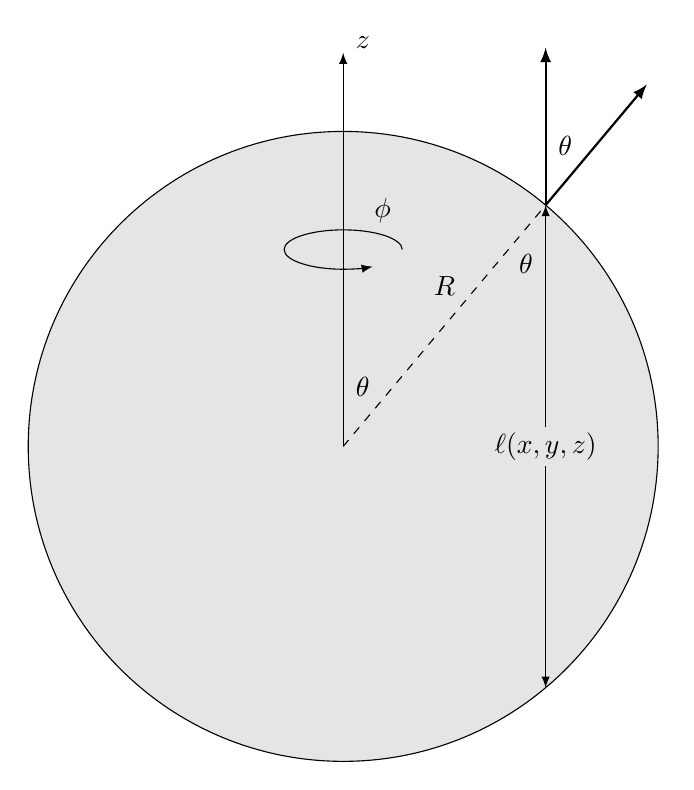
\begin{tikzpicture}
  \draw[fill=gray!20] (0,0) circle (4cm);
  \draw[-latex] (0,0) -- (0,5);
%  \draw[-latex] (0, 2.5) ellipse [x radius = 0.75cm, y radius = 0.25cm, start angle = -70, end angle = 250];
  \draw[-latex] (0.75,2.5) arc (0:300:0.75cm and 0.25cm); 
  \node at (0.5,3) {$\phi$};
  \node at (0.25,5.125) {$z$};
  \draw[dashed] (0,0) -- ({4*cos(50)},{4*sin(50)});
  \node at (0.25,0.75) {$\theta$};
  \node at ({2*cos(50)},{2*sin(50) + 0.5}) {$R$};
  \draw[thick,-latex] ({4*cos(50)},{4*sin(50)}) -- +({2*cos(50)},{2*sin(50)});
  \node at ({6*cos(50) + 0.125},{6*sin(50) - 0.25}) {$\rhat$};
  \draw[thick,-latex] ({4*cos(50)},{4*sin(50)}) -- +(0,2);
  \node at ({4*cos(50) - 0.25},{4*sin(50) + 2}) {$\khat$};
  \node at ({4*cos(50) + 0.25},{4*sin(50) + 0.75}) {$\theta$};
  \node at ({4*cos(50) - 0.25},{4*sin(50) - 0.75}) {$\theta$};
  \node at ({4*cos(50)},0) {$\ell(x,y,z)$};
  \draw[-latex] ({4*cos(50)},0.25) -- ({4*cos(50)},{4*sin(50)});
  \draw[-latex] ({4*cos(50)},-0.25) -- ({4*cos(50)},{-4*sin(50)});
\end{tikzpicture}
\caption{Illustration of the problem setup for the escape probability from a radioactive sphere.}
\label{Fig:vector_escapeProbabilitySphere}
\end{center}
\end{figure}

The escape probability can be written as the ratio of the rate photons escape the sphere divided by the total rate they are emitted in the sphere. If the emission rate density is $Q_0$ photons per unit volume per unit time and the sphere has a volume $V$, then the total emission rate is $Q_0 V$. The rate photons escape is given by
\begin{align}
  \int_S \mathbf{J} \cdot d\mathbf{S}.
\end{align}
Here $\mathbf{J}$ is a vector field describing the photon current. Because of spherical symmetry, we may always work the problem such that the $z$ axis is always aligned in the direction of photon flight. When we do this, we may express the photon current vector field as
\begin{align}
  \mathbf{J} = \frac{Q_0}{\Sigma_t} \left[ 1 - \exp \left( -\Sigma_t \ell(x,y,z) \right) \right] \khat .
\end{align}
Here $\ell(x,y,z)$ is the length of a chord along the $z$ direction from one end of the sphere to the other. The escape probability becomes
\begin{align}
  p_{esc} &= \frac{1}{Q_0 V} \int_S \frac{Q_0}{\Sigma_t} \left[ 1 - \exp \left( -\Sigma_t \ell(x,y,z) \right) \right] \khat \cdot d\mathbf{S} \nonumber \\
          &= \frac{1}{\Sigma_t V} \int_S \left[  1 - \exp \left( -\Sigma_t \ell(x,y,z) \right) \right] \khat \cdot d\mathbf{S}
\end{align}
Since all of the photons travel in the $+z$ direction, the photons only leak out of the northern hemisphere of the sphere. For this, we will integrate over the $\theta$-$\phi$ plane in spherical coordinates. The integral over the northern hemisphere becomes:
\begin{align}
  p_{esc} &= \frac{1}{\Sigma_t V} \int_0^{2\pi} \int_0^{\pi/2} \left[  1 - \exp \left( -\Sigma_t \ell(x,y,z) \right) \right] \khat \cdot ( R^2 \sin\theta \rhat  ) d\theta d\phi .
\end{align}
From the diagram, we can see that 
\begin{align}
  \khat \cdot \rhat = \cos \theta .
\end{align}
The chord length is
\begin{align}
  \ell(x,y,z) = 2 z = 2 R \cos \theta.
\end{align}
Inserting this into the integral gives
\begin{align}
  p_{esc} &= \frac{R^2}{\Sigma_t V} \int_0^{2\pi} \int_0^{\pi/2} \left[  1 - \exp \left( -2 \Sigma_t R \cos \theta \right) \right] \cos \theta \sin\theta d\theta d\phi .
\end{align}
The azimuthal angle can be integrated trivially:
\begin{align}
  p_{esc} &= \frac{2 \pi R^2}{\Sigma_t V} \int_0^{\pi/2} \left[  1 - \exp \left( -2 \Sigma_t R \cos \theta \right) \right] \cos \theta \sin\theta d\theta .
\end{align}
To carry out the polar integral, introduce the transformation
\begin{subequations}
\begin{align}
   \mu &= \cos \theta , \\
   d\mu &= -\sin \theta d \theta .
\end{align}
\end{subequations}
After making this transformation:
\begin{align}
  p_{esc} &= \frac{2 \pi R^2}{\Sigma_t V} \int_0^1 \left[  1 - \exp \left( -2 \Sigma_t R \mu \right) \right] \mu d \mu .
\end{align}
After carrying out the integrals (integrate by parts) we get
\begin{align}
  p_{esc} &= \frac{2\pi R^2}{\Sigma_t V} \left[  \frac{1}{2} -  \frac{ 1 - ( 1 + 2 \Sigma_t R ) e^{-2 \Sigma_t R}  }{  4 \Sigma_t^2 R^2 } \right] .
\end{align}
After some rearrangement and expanding out the volume of a sphere,
\begin{align}
  p_{esc} &= \frac{3}{8 \Sigma_t^3  R^3} \bigg[  2 \Sigma_t^2 R^2 - 1  + ( 1 + 2 \Sigma_t R ) e^{-2 \Sigma_t R } \bigg] .
\end{align}
It is often convenient to express the result in terms of the optical radius
\begin{align}
  \tau = \Sigma_t R,
\end{align}
which gives the final result
\begin{align}
  p_{esc} &= \frac{3}{8 \tau^3} \bigg[ ( 1 + 2 \tau ) e^{-2\tau} + 2 \tau^2 - 1 \bigg] .
\end{align}


%%%%%%%%%%%%%%%%%%%%%%%%%%%%%%%%%%%%%%%%%%%%%%%%%%%%%%%%%%%%%%%%%%%%%%%%%%%%%%%%%%%%%%%%%%%%%%%
%%%%%%%%%%%%%%%%%%%%%%%%%%%%%%%%%%%%%%%%%%%%%%%%%%%%%%%%%%%%%%%%%%%%%%%%%%%%%%%%%%%%%%%%%%%%%%%
\section{Volume Integrals}

The final related quantity to vector analysis is the concept of a volume integral. Most commonly, volume integrals are performed upon some density field of some quantity per unit volume to find the number of that quantity within some region. This is given as
\begin{align}
  \int_V \rho(\pos) dV .
\end{align}
Here $dV$ is the differential volume, which gets expanded out as a triple differential.

As mentioned in the previous section on surface integrals, the volume integral of the divergence of a vector field can also be related to the surface integral of the net outgoing flux of a physical quantity for that same field. This will be discussed later in the chapter.


%%%%%%%%%%%%%%%%%%%%%%%%%%%%%%%%%%%%%%%%%%%%%%%%%%%%%%%%%%%%%%%%%%%%%%%%%%%%%%%%%%%%%%%%%%%%%%%
\subsection{Differential Volume}

The differential volume $dV$ is a scalar quantity that can be obtained generally by taking the determinant of the Jacobian matrix
\begin{align}
  dV = \det{ J } du dv dw.
\end{align}
An equivalent formulation for orthogonal coordinate systems is the product of the scale factors times the differential elements of each coordinate:
\begin{align}
  dV = h_u h_v h_w du dv dw.
\end{align}
For Cartesian, cylindrical, and spherical coordinates, the differential volume element becomes
\begin{subequations}
\begin{align}
  dV &= dx dy dz, \\
  dV &= r dr d\theta dz, \\
  dV &= r^2 \sin \theta dr d\theta d\phi .
\end{align}
\end{subequations}


%%%%%%%%%%%%%%%%%%%%%%%%%%%%%%%%%%%%%%%%%%%%%%%%%%%%%%%%%%%%%%%%%%%%%%%%%%%%%%%%%%%%%%%%%%%%%%%
\subsection{Example: Enclosed Charge in a Cylinder}

In electrostatics calculations of the electric field, we often compute the charge enclosed by a given volume $Q_{enc}$ with a prescribed charge density $\rho$. The approach is to simply integrate the charge density over the region.

Suppose we have a charge density given in a cylindrical region:
\begin{align}
  \rho(r,\theta,z) = \left\{ \begin{array}{l l} 
    \rho_0 e^{-\kappa r^2 }, & \quad 0 \le r \le R, \  0 \le \theta < 2\pi, \  0 \le z \le H \\
    0, & \quad \text{otherwise} \\ \end{array} \right. .
\end{align}
The charge enclosed by this region may be obtained by integrating over the region (or any region larger than it). This is:
\begin{align}
  Q_{enc} &= \int_V \rho_0 e^{-\kappa r^2 } dV \nonumber \\
  &= \int_0^H \int_0^{2\pi} \int_0^R \rho_0 e^{-\kappa r^2 } r dr d\theta dz .
\end{align}
Carrying out the $\theta$ and $z$ integrals is trivial, yielding
\begin{align}
  Q_{enc} &= 2\pi H \rho_0 \int_0^R  r e^{-\kappa r^2 } dr .
\end{align}
Performing the integral over $r$ using integration by parts gives the final result:
\begin{align}
  Q_{enc} &= \frac{\pi H \rho_0}{\kappa} ( 1 - e^{-\kappa R^2} ).
\end{align}

%%%%%%%%%%%%%%%%%%%%%%%%%%%%%%%%%%%%%%%%%%%%%%%%%%%%%%%%%%%%%%%%%%%%%%%%%%%%%%%%%%%%%%%%%%%%%%%%
%%%%%%%%%%%%%%%%%%%%%%%%%%%%%%%%%%%%%%%%%%%%%%%%%%%%%%%%%%%%%%%%%%%%%%%%%%%%%%%%%%%%%%%%%%%%%%%%
\section{Integral Theorems}

In vector calculus we have three major integral theorems that, in many circumstances, allow us to greatly simplify problems or show equivalences between quantities of interest. The first is the gradient theorem, which is useful in defining conservative forces or scalar potential functions, which allows us to take a line integral of a vector field as simply the scalar potential evaluated at the endpoints. The second is the divergence theorem, which relates volume and surface integrals. And the third is Stokes' theorem, which relates surface and line integrals.

%%%%%%%%%%%%%%%%%%%%%%%%%%%%%%%%%%%%%%%%%%%%%%%%%%%%%%%%%%%%%%%%%%%%%%%%%%%%%%%%%%%%%%%%%%%%%%%%
\subsection{Gradient Theorem}

The gradient theorem, which is analogous to the second fundamental theorem of calculus, but allied to line integrals states that
\begin{align}
  \int_{P(a,b)} \nabla f \cdot d\boldsymbol\ell = f(P(b)) - f(P(a)) .
\end{align}
This states that if a vector field is described by a gradient of a function, then we can assert that the line integral only depends upon the endpoints. Note that since the curl of the gradient is always zero, this implies that if we have some vector field $\mathbf{F}$ and if $\nabla \times \mathbf{F} = \mathbf{0}$, then the line integral of that vector field is path independent. We state that the vector field $\mathbf{F}$ is conservative. This result will be used in our discussion on potential functions in the following section.

%%%%%%%%%%%%%%%%%%%%%%%%%%%%%%%%%%%%%%%%%%%%%%%%%%%%%%%%%%%%%%%%%%%%%%%%%%%%%%%%%%%%%%%%%%%%%%%%
\subsection{Divergence Theorem}

The divergence theorem relates volume and surface integrals. It states that the divergence of some vector field integrated over a convex volume is equal to the surface integral of the vector field over the surface bounding that volume. In other words,
\begin{align}
  \oint_S \mathbf{F} \cdot d\mathbf{S} = \int_V \nabla \cdot \mathbf{F} dV.
\end{align}

The idea with the divergence theorem starts from the interpretation of $(\nabla \cdot \mathbf{F})dV$ is the net outflow of a physical quantity given by vector field $\mathbf{F}$ out of some convex differential volume $dV$ about $(x,y,z)$. For a six sided cubic differential volume, we may express this as:
\begin{align}
  ( \nabla \cdot \mathbf{F} ) dV_1 
  &= \text{ outflow across faces of $dV_1$  } - \text{ inflow across faces of $dV_1$  }  .
\end{align}
If we then stack a differential volume $dV_2$ next to $dV_1$ such that the face $\circled{2}$ of $dV_1$ is adjacent to $\circled{1}$ of $dV_2$ and add the two together we get
\begin{align}
  &( \nabla \cdot \mathbf{F} ) dV_1 + ( \nabla \cdot \mathbf{F} ) dV_2 \nonumber \\
  &= \text{ outflow across face \circled{2} of $dV_1$ } \nonumber \\
  &- \text{ inflow across face \circled{2} of $dV_1$ } \nonumber \\
  &+ \text{ outflow across exterior faces $dV_1$  } - \text{ inflow across exterior faces of $dV_1$  } \nonumber \\
  &+ \text{ outflow across face \circled{1} of $dV_2$  } \nonumber \\
  &- \text{ inflow across face \circled{1} of $dV_2$ } \nonumber \\
  &+ \text{ outflow across exterior faces $dV_2$  } - \text{ inflow across exterior faces of $dV_2$  } .
\end{align}
Since there are no particles created on the face, we can assert the continuity condition that
\begin{subequations}
\begin{align}
   &\text{ outflow across face \circled{2} of $dV_1$   } = \text{ inflow across face \circled{1} of $dV_2$ } , \\
   &\text{ inflow across face \circled{2} of $dV_1$   } = \text{ outflow across face \circled{1} of $dV_2$ } .
\end{align}
\end{subequations}
Therefore, the terms cancel and we are left with
\begin{align}
  &( \nabla \cdot \mathbf{F} ) dV_1 + ( \nabla \cdot \mathbf{F} ) dV_2 \nonumber \\
  &= \text{ outflow across exterior faces $dV_1$  } - \text{ inflow across exterior faces of $dV_1$  } \nonumber \\
  &+ \text{ outflow across exterior faces $dV_2$  } - \text{ inflow across exterior faces of $dV_2$  } .
\end{align}
If we add another set of differential volumes such that the net volume remains convex so as not to permit reentry, we have the same result that only the exterior faces remain. Since adding over numerous differentials limits to an integral, we get the result that 
\begin{align}
  \lim_{k \rightarrow \infty} \sum_k ( \nabla \cdot \mathbf{F} ) dV_k &= \int_V \nabla \cdot \mathbf{F} dV \nonumber \\ 
  &= \text{ outflow across the exterior boundary of $V$ } \nonumber \\ &- \text{ inflow across the exterior boundary of $V$ } .
\end{align}

Now, if we inspect the surface integral, we note that the differential surface vector $d\mathbf{S} = \nhat dS$, where the normal vector $\nhat$ is defined by convention to be pointed outward from the surface. When $\mathbf{F} \cdot \nhat > 0$ we have outward directed flow (positive) across the surface and when $\mathbf{F} \cdot \nhat < 0$ we have inward directed flow (negative) across, which is equivalent to the volume integral of the divergence.


%%%%%%%%%%%%%%%%%%%%%%%%%%%%%%%%%%%%%%%%%%%%%%%%%%%%%%%%%%%%%%%%%%%%%%%%%%%%%%%%%%%%%%%%%%%%%%%%
\subsection{Stokes' (Curl) Theorem}

Stoke's theorem states the line integral of a vector field along a closed path is equal to the curl of that vector field integrated over some some smooth surface that is bounded by the path. This is stated mathematically as
\begin{align}
  \oint_P \mathbf{F} \cdot d\boldsymbol\ell = \int_S ( \nabla \times \mathbf{F} ) \cdot d\mathbf{S} .
\end{align}

While the idea is more abstract than the divergence theorem, the argument proceeds along similar lines. The curl of a vector field gives the local circulation of some differential patch of area about some point $(x,y,z)$ with an outward normal vector $\nhat$. This circulation is often represented with some outward unit normal that describes counter-clockwise rotation with respect to that outward normal. If we take another path of area adjacent, we have another counter-clockwise rotation. As with the divergence theorem, the counter-clockwise rotation of one side is canceled by the counter-clockwise rotation of the other side since the rotation vectors are opposite of one another. This leaves only the rotation about the exterior of the combined surface. As with the divergence theorem, if we continue to stack patches of adjacent area and add them up, the limiting result is a line integral over the bounding curve.


%%%%%%%%%%%%%%%%%%%%%%%%%%%%%%%%%%%%%%%%%%%%%%%%%%%%%%%%%%%%%%%%%%%%%%%%%%%%%%%%%%%%%%%%%%%%%%%%
\subsection{Example: Maxwell's Equations of Electromagnetism}

Maxwell's equations of electromagnetism can be written in equivalent differential and integral forms. Depending upon the context, working with one of these formulations over the other may produce a problem that is easier to solve.

The first of Maxwell's equations states that the divergence of the electric field is equal to the local charge density divided by the electric permittivity:
\begin{align}
  \nabla \cdot \mathbf{E} = \frac{\rho}{\epsilon_0}.
\end{align}
If we integrate the left hand side over a closed, convex volume, we can write
\begin{align}
  \int_V ( \nabla \cdot \mathbf{E} ) dV = \int_V \frac{\rho}{\epsilon_0} dV = \frac{Q_{enc}}{\epsilon_0} .%\oint_S \mathbf{E} \cdot d\mathbf{S} 
\end{align}
The right-hand side becomes the total net charge enclosed by the volume. By applying the divergence theorem we get
\begin{align}
  \int_V ( \nabla \cdot \mathbf{E} ) dV = \oint_S \mathbf{E} \cdot d\mathbf{S} = \frac{Q_{enc}}{\epsilon_0} .
\end{align}

Faraday's law states that the curl of the electric field is equal to the negative time rate of change of the magnetic field:
\begin{align}
  \nabla \times \mathbf{E} = -\dho{\mathbf{B}}{t} .
\end{align}
Taking the integral over some non-closed surface of this gives
\begin{align}
  \int_S ( \nabla \times \mathbf{E} ) \cdot d\mathbf{S} = -\dho{}{t} \int_S \mathbf{B} \cdot d\mathbf{S} = -\dho{\Phi_B}{t} .
\end{align}
The right-hand side becomes the time-rate of change of the magnetic flux. Applying Stokes' theorem gives
\begin{align}
  \int_S ( \nabla \times \mathbf{E} ) \cdot d\mathbf{S} = \oint_{P} \mathbf{E} \cdot d\boldsymbol\ell = -\dho{\Phi_B}{t} .
\end{align}
This states that the integral over a closed path of the electric field vector is equivalent to minus to the time rate of change of the magnetic flux across any smooth surface bounded by that curve.

The nonexistence of magnetic monopoles (point sources of magnetic charge) implies that the divergence of the magnetic field is zero:
\begin{align}
  \nabla \cdot \mathbf{B} = 0.
\end{align}
As with Gauss' law for electric fields, we integrate this equation over the volume and apply the divergence theorem:
\begin{align}
  \int_V ( \nabla \cdot \mathbf{B} ) dV = \oint_S \mathbf{B} \cdot d\mathbf{S} = 0 .
\end{align}
This states that if we integrate the magnetic field over any closed surface, we will get zero. In other words, there is never a net outward directed magnetic flux out of a volume.

Finally, we have Ampere's law (with Maxwell's correction) that relates the curl of the magnetic field with the current and time rate of change of the electric field:
\begin{align}
  \nabla \times \mathbf{B} = \mu_0 \left( \mathbf{J} + \epsilon_0 \dho{\mathbf{E}}{t} \right).
\end{align}
Here $\mu_0$ is the magnetic permeability of free space. If, as we did with Faraday's law, we proceed to take the surface integral over some non-closed surface, we get
\begin{align}
  \int_S ( \nabla \times \mathbf{B} ) \cdot d \mathbf{S} = \mu_0 \left( \int_S \mathbf{J} \cdot d\mathbf{S} 
  + \epsilon_0 \dho{}{t} \left( \int_S \mathbf{E} \cdot d\mathbf{S} \right) \right).
\end{align}
Applying Stoke's theorem gives
\begin{align}
  \int_S ( \nabla \times \mathbf{B} ) \cdot d \mathbf{S} = \oint_P \mathbf{B} \cdot d\boldsymbol\ell = \mu_0 \left( \int_S \mathbf{J} \cdot d\mathbf{S} 
  + \epsilon_0 \dho{\Phi_E}{t}  \right).
\end{align}
This states that the line integral over a closed path of the magnetic field is equal to the sum of the current flowing across the surface plus the time rate of change of the electric flux.

%%%%%%%%%%%%%%%%%%%%%%%%%%%%%%%%%%%%%%%%%%%%%%%%%%%%%%%%%%%%%%%%%%%%%%%%%%%%%%%%%%%%%%%%%%%%%%%
%%%%%%%%%%%%%%%%%%%%%%%%%%%%%%%%%%%%%%%%%%%%%%%%%%%%%%%%%%%%%%%%%%%%%%%%%%%%%%%%%%%%%%%%%%%%%%%
\section{Potential Functions}

A useful mathematical object for describing vector fields is the potential function. These come in two flavors, a scalar potential $\Phi$ and a vector potential $\mathbf{A}$. Note that while these are sometimes similar to the concept of potential energy from classical mechanics, the two concepts are fundamentally different and should not be confused. This is an unfortunate naming convention, but is unavoidable. The advantage of casting vector fields in terms of potentials is that they can make the mathematics of performing line and surface integrals much simpler. In the context of line integration, it also allows us to express the idea in terms of curves within covector fields.

%%%%%%%%%%%%%%%%%%%%%%%%%%%%%%%%%%%%%%%%%%%%%%%%%%%%%%%%%%%%%%%%%%%%%%%%%%%%%%%%%%%%%%%%%%%%%%%
\subsection{Helmholtz Decomposition}

The Helmholtz decomposition theorem (also called the fundamental theorem of vector analysis) states that any vector field that is at least differentiable twice everywhere (corresponding to most vector fields in physics) may be written as the the sum of the gradient of a scalar function and the curl of another function:
\begin{align}
  \mathbf{F} = -\nabla \Phi + \nabla \times \mathbf{A} .
\end{align}
Here we call $\Phi$ the scalar potential function and $\mathbf{A}$ the vector potential function. Note that the minus sign on the $\nabla \Phi$ term is purely because of an arbitrary convention and not inherent in the mathematics.

Why this decomposition is useful is that we can often write differential equations or integrals involving unknown vector fields in terms of the potential functions instead. The resulting differential equations or integrals are often much easier to solve. Once we know the potential functions, we can use the relationship to obtain the unknown vector field.


%If we take the divergence of the vector field and note that the divergence of the curl is zero:
%\begin{align}
%  \nabla \cdot \mathbf{F} = -\nabla \cdot \nabla \Phi + \nabla \cdot \nabla \times \mathbf{A} = -\nabla^2 \Phi.
%\end{align}
%Alternatively, 


%Vector fields with $\nabla \cdot \mathbf{F} = 0$ are referred to as solenoidal and can be described using the vector potential $\mathbf{A}$ alone. The most common example in physics of such a field is the magnetic field, which always satisfied $\nabla \cdot \mathbf{B} = 0$. 


%%%%%%%%%%%%%%%%%%%%%%%%%%%%%%%%%%%%%%%%%%%%%%%%%%%%%%%%%%%%%%%%%%%%%%%%%%%%%%%%%%%%%%%%%%%%%%%
\subsection{Scalar Potential Function}

Vector fields satisfying $\nabla \times \mathbf{F} = \mathbf{0}$ are called irrotational or conservative and can be described using the scalar potential $\Phi$ alone, i.e.,
\begin{align}
  \mathbf{F} = -\nabla \Phi, \quad \text{ if } \nabla \times \mathbf{F} = \mathbf{0}.
\end{align}
Examples of irrotational vector fields include the gravitational field and the electric field in the absence of time-varying magnetic fields. 

Then the curl of a vector field zero, we can also state that the line integral depends only upon the potential function at the endpoints:
\begin{align}
  \int_{P(a,b)} \mathbf{F} \cdot d\boldsymbol\ell = \Phi(a) - \Phi(b) .
\end{align}
Correspondingly, it follows that if the path is over a closed loop then,
\begin{align}
  \oint_{P} \mathbf{F} \cdot d\boldsymbol\ell = 0 .
\end{align}

To demonstrate this, the line integral may be written as
\begin{align}
  - \int_{P(a,b)} \nabla \Phi \cdot d\boldsymbol\ell .
\end{align}
Suppose the path is parameterized by $t$. We can then use the chain rule to write
\begin{align}
  - \int_{P(a,b)} \nabla \Phi \cdot \frac{d\boldsymbol\ell}{dt} dt .
\end{align}
The gradient of the potential field can be expanded in Cartesian coordinates as
\begin{align}
  \nabla \Phi = \dho{\Phi}{x} \ihat + \dho{\Phi}{y} \jhat + \dho{\Phi}{x} \khat .
\end{align}
(The result applies to any coordinate system, but the choice of Cartesian coordinates simplifies the derivation.) We can then expand the derivative of the line vector with respect to the parameter $t$ ranging along the path from $a \le t \le b$ using the multivariable chain rule:
\begin{align}
  \frac{d\boldsymbol\ell}{dt} = \dho{x}{t} \dho{\boldsymbol\ell}{x} + \dho{y}{t} \dho{\boldsymbol\ell}{y} + \dho{z}{t} \dho{\boldsymbol\ell}{z} .
\end{align}
Since $\boldsymbol\ell$ represents a displacement vector, its partial derivatives are simply the Cartesian basis vectors:
\begin{align}
  \frac{d\boldsymbol\ell}{dt} = \dho{x}{t} \ihat + \dho{y}{t} \jhat + \dho{z}{t} \khat .
\end{align}
Evaluating the dot product gives
\begin{align}
  \nabla \Phi \cdot \frac{d\boldsymbol\ell}{dt} = \dho{\Phi}{x} \dho{x}{t} + \dho{\Phi}{y} \dho{y}{t} + \dho{\Phi}{z} \dho{z}{t} .
\end{align}
The right-hand side can be simplified by applying the multivariable chain rule in reverse:
\begin{align}
  \frac{ d \Phi }{ dt } = \dho{\Phi}{x} \dho{x}{t} + \dho{\Phi}{y} \dho{y}{t} + \dho{\Phi}{z} \dho{z}{t} = \nabla \Phi \cdot \frac{d\boldsymbol\ell}{dt}.
\end{align}
Therefore, we can rewrite the integral as
\begin{align}
  - \int_a^b \frac{ d \Phi }{ dt } dt .
\end{align}
The $dt$ can be cancelled and the integral can be carried out trivially:
\begin{align}
  - \int_a^b d \Phi = \Phi(a) - \Phi(b) .
\end{align}

An important point is that the scalar function $\Phi$ is not unique. Suppose instead we let
\begin{align}
  \Phi = \Phi_0 + C
\end{align}
where $C$ is an arbitrary scalar constant. Because the gradient of a constant is the same, we get the same result, i.e.,
\begin{align}
  \mathbf{F} = \nabla \Phi = \nabla ( \Phi_0 + C ) = \nabla \Phi_0 .
\end{align}
While the potential function is not the potential energy, it does have the same feature (which is the source of much confusion) that where the potential equals zero is entirely arbitrary and defined as a matter of convenience. Regardless of where the zero point is defined, the physics will work out entirely the same.

Before continuing, it may seems a bit odd that a single scalar function $\Phi$ can encode enough information to describe the three components of a vector field $\mathbf{F} = -\nabla \Phi$. Note that, however, the $F_x$, $F_y$, and $F_z$ components are not independent, because $\nabla \times \mathbf{F} = \mathbf{0}$. In other words,
\begin{align}
  \dho{F_z}{y} = \dho{F_y}{z}, \nonumber \\
  \dho{F_z}{x} = \dho{F_x}{z}, \nonumber \\
  \dho{F_y}{x} = \dho{F_x}{y}. \nonumber
\end{align}


%%%%%%%%%%%%%%%%%%%%%%%%%%%%%%%%%%%%%%%%%%%%%%%%%%%%%%%%%%%%%%%%%%%%%%%%%%%%%%%%%%%%%%%%%%%%%%%
\subsection{Relation to Covector Fields}

Recall that the line integral of the a conservative force field reduces to 
\begin{align}
  \int_{P(a,b)} \mathbf{F} \cdot d\boldsymbol\ell = - \int_{P(a,b)} d \Phi = \Phi(a) - \Phi(b) .
\end{align}
Recall that the differential operator $d$ acting upon a scalar field $\Phi$ produces a covector field, which can be represented as a series of contour lines of equal potential. To illustrate, let us consider the electric potential from a point charge with charge $Q$ at the origin in spherical coordinates:
\begin{align}
  \Phi = \frac{1}{4\pi\epsilon_0} \frac{Q}{r} .
\end{align}
Here the potential function is defined to be zero as $r \rightarrow \infty$, but we could add or subtract any arbitrary constant and get identical results. 

The covector field $d\Phi$ can be computed using the multivariable chain rule
\begin{align}
  d\Phi &= \dho{\Phi}{r} dr + \dho{\Phi}{\theta} d\theta + \dho{\Phi}{\phi} d\phi \nonumber \\
  &= -\frac{1}{4\pi \epsilon_0} \frac{Q}{r^2} dr .
\end{align}
This covector can be multiplied by a vector of coordinates and set equal to some constant $a$:
\begin{align}
  \left[ \begin{array}{c c c} -\dfrac{1}{4\pi \epsilon_0} \dfrac{Q}{r^2} & 0 & 0 \\ \end{array} \right]
  \left[ \begin{array}{c} r \\ \theta \\ \phi \\ \end{array} \right] = -\dfrac{1}{4\pi \epsilon_0} \dfrac{Q}{r} = a .
\end{align}
This gives a series of spherical surfaces of equal potential that become increasingly close together nearing the origin and spacing further apart the further away. Each spherical surface of equal potential also has an outward directed orientation giving the negative direction of increasing potential. A 2-D slice of these surfaces is taken along the origin to make a series of circles with arrows describing the orientation: this is illustrated in Fig.~\ref{Fig:vector_covectorContoursElectrostaticPotential}.

\begin{figure}[tb!]
\begin{center}
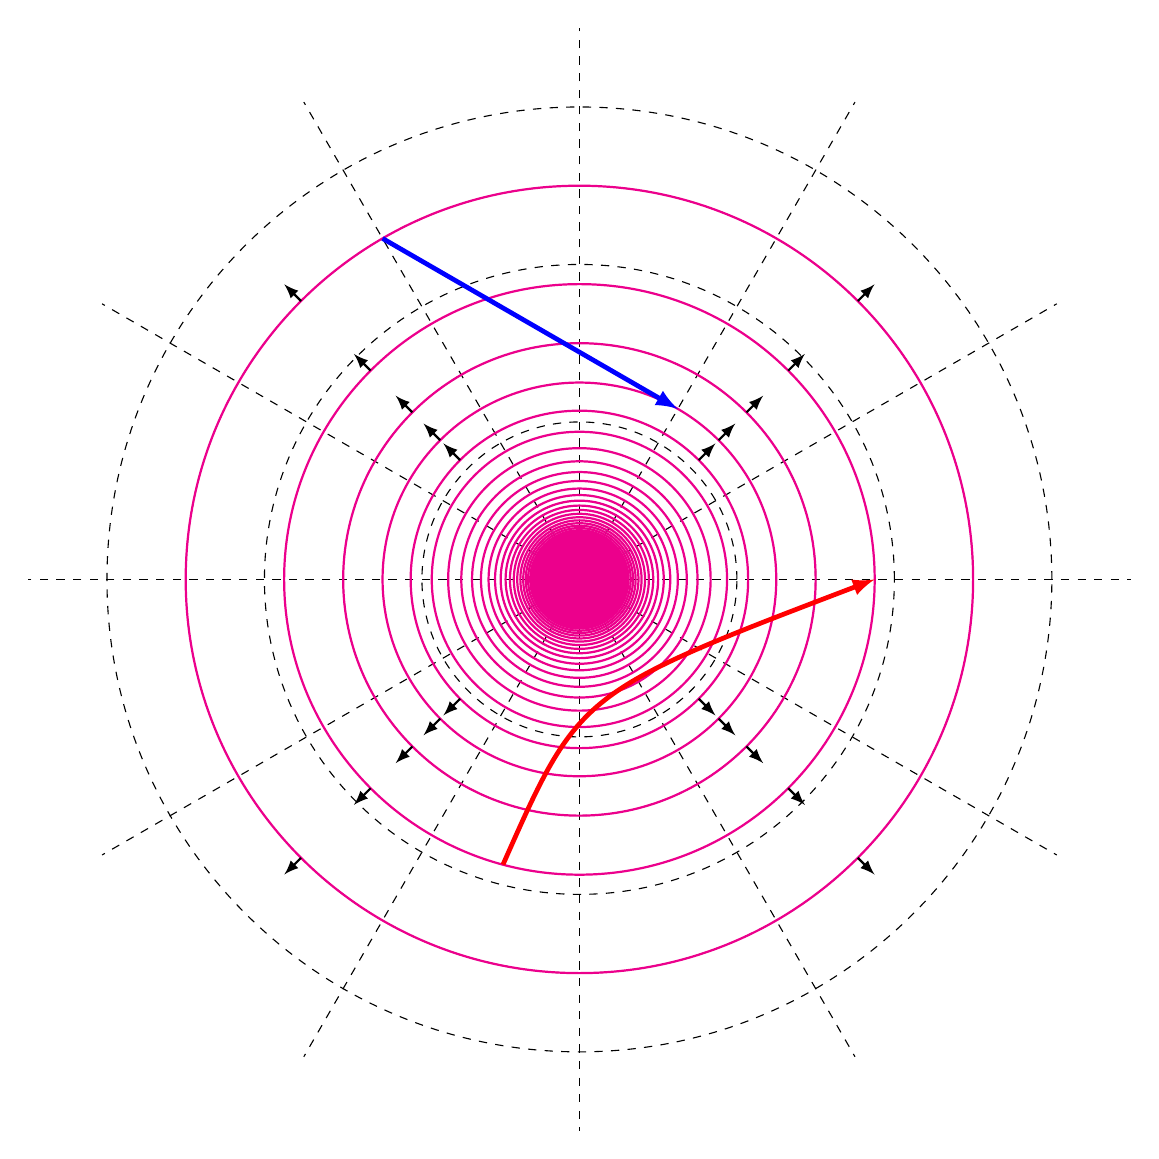
\begin{tikzpicture}
  \foreach \r in {1,...,6} 
     \draw[dashed] (0,0) circle (\r);
  \foreach \t in {0, 30, 60, 90, 120, 150, 180, 210, 240, 270, 300, 330}
     \draw[dashed] (0,0) -- ({7*cos(\t)},{7*sin(\t)});
  \foreach \a in {3,...,24}
     \draw[thick, color=magenta] (0,0) circle ({15/\a});
  \fill[magenta] (0,0) circle (0.625);

  \foreach \t in {45,135,225,315} {
    \foreach \a in {3,...,7} {
      \draw[-latex,thick] ({15*cos(\t)/\a},{15*sin(\t)/\a}) -- +({0.3*cos(\t)},{0.3*sin(\t)});
    }
  }
  
  \draw[-latex,color=blue,line width=0.6mm] ({15/3*cos(120)},{15/3*sin(120)}) -- ({15/6*cos(60)},{15/6*sin(60)});
  \draw[-latex,color=red,line width=0.6mm] ({15/4*cos(255)},{15/4*sin(255)}) .. controls ({15/10.5*cos(270)},{15/10.5*sin(270)}) .. ({15/4},0);
\end{tikzpicture}
\caption{Illustration of contour curves for the electrostatic potential from a point charge at the origin and two different paths for another charged particle.}
\label{Fig:vector_covectorContoursElectrostaticPotential}
\end{center}
\end{figure}

The electric potential is related to the electric field by minus the gradient of the potential
\begin{align}
  \mathbf{E} = -\nabla \Phi .
\end{align}
The force done on a particle of charge $q$ by an electrostatic field is
\begin{align}
  \mathbf{F} = q \mathbf{E} = -q \nabla \Phi.
\end{align}
Therefore, the work done by an electrostatic field for the charged particle moving along path $P(a,b)$ is
\begin{align}
  W = -q \int_{P(a,b)}  \nabla \Phi \cdot d\boldsymbol\ell = -q \int_a^b d \Phi = q \left( \Phi(a) - \Phi(b) \right) .
\end{align}

In a similar manner to when a covector field acts upon a vector and produces a scalar, here the covector field $d \Phi$ acts upon each differential increment of path to produce some differential increment of work and the integral sums over the result to give the total work. In a similar manner, the work (per unit charge $q$) can be obtained by counting the number of covector contour lines that the path pierces considering the orientation of those contour lines. 

The straight line path in blue displayed in Fig.~\ref{Fig:vector_covectorContoursElectrostaticPotential} shows the work per unit charge $q$ by counting the number of lines crossed is $-3$. If the two charges $q$ and $Q$ have the same sign, the charges will repel one another and the work done by will be negative since energy must be added by the charge $q$ to reach the surface. Likewise, if the charges have opposite signs, the charge $q$ will be attracted to the origin and the work will be positive.

The curved path in red displayed in Fig.~\ref{Fig:vector_covectorContoursElectrostaticPotential} has a work per charge of zero since the positive and negative lines crossed are equal and the work cancels. In other words, the particle begins and ends at the same distance away from the origin. For a charge $q$ with the same sign as $Q$, the field does work against the particle (negative) initially going inward and then does work (positive) on the particle moving outward.


%%%%%%%%%%%%%%%%%%%%%%%%%%%%%%%%%%%%%%%%%%%%%%%%%%%%%%%%%%%%%%%%%%%%%%%%%%%%%%%%%%%%%%%%%%%%%%%
\subsection{Vector Potential Function}

Physical vector field quantities for which the curl is nonzero cannot be described using the gradient of a scalar potential function. Vector fields that are divergence free or solenoidal (e.g., magnetic fields or fluids that are purely rotational) can be described by the curl of a vector potential $\mathbf{A}$. Mathematically,
\begin{align}
  \mathbf{F} = \nabla \times \mathbf{A}, \quad \text{ if } \nabla \cdot \mathbf{F} = 0.
\end{align}
This result arises from the vector identity that the divergence of the curl of a vector field is zero.

Analogous to the scalar potential function, the vector potential function is unique to within a gradient of a scalar field. Suppose we write
\begin{align}
  \mathbf{A} = \mathbf{A}_0 + \nabla m .
\end{align} 
Taking the curl gives
\begin{align}
  \mathbf{F} = \nabla \times \mathbf{A} = \nabla \times \mathbf{A}_0 + \nabla \times \nabla m = \nabla \times \mathbf{A}_0 .
\end{align}
The term $\nabla \times \nabla m = \mathbf{0}$ since the curl of the gradient is always zero.

Unlike with the scalar potential, which is unique to within an additive constant, the addition of a function is not a trivial matter. While the choice of $\nabla m$ will not impact the final result, different choices may make the calculations significantly easier or more difficult. The selection of $\nabla m$ is called \emph{gauge fixing} and is a challenge to enable theoretical calculations involving physical quantities. Also note that like the scalar potential function, the vector potential function is not by itself a physical quantity; rather, it is a useful mathematical quantity that can be used to obtain physical quantities.

%%%%%%%%%%%%%%%%%%%%%%%%%%%%%%%%%%%%%%%%%%%%%%%%%%%%%%%%%%%%%%%%%%%%%%%%%%%%%%%%%%%%%%%%%%%%%%%
\subsection{Example: Electric and Magnetic Potential Functions}

Continuing to apply vector calculus to electromagnetism and Maxwell's equations, we first begin with Gauss' law of electric fields, which, in its differential form, states
\begin{align}
  \nabla \cdot \mathbf{E} = \frac{\rho}{\epsilon_0} . \nonumber
\end{align}
Expanding out the terms yields a first-order partial differential equation that can actually be difficult to solve. Perhaps unexpectedly, since it would result in a second-order partial differential equation, it is easier to solve this problem if we insert the electric potential. For this, we assume that the fields are static, i.e., not time varying, so that $\nabla \times \mathbf{E} = \mathbf{0}$ from Faraday's law. This gives
\begin{align}
  \nabla \cdot (-\nabla \Phi) = -\nabla^2 \Phi = \frac{\rho}{\epsilon_0} .
\end{align}
This equation is referred to as Poisson's equation. In the case where the charge density $\rho$ is zero and the electric potential is specified at the boundaries, as is often the case, we have Laplace's equation. These second-order partial differential equations have mathematical properties that lend themselves to both analytical and numerical solution. Once we have $\Phi$, we can easily determine the electric field $\mathbf{E}$ by taking $-\nabla \Phi$.

To show the magnetic potential, we begin with Ampere's law with a time-independent electric field
\begin{align}
  \nabla \times \mathbf{B} = \mu_0 \mathbf{J} . \nonumber
\end{align}
Since the magnetic field $\mathbf{B}$ is always solenoidal because there are no point charges of magnetism, i.e., $\nabla \cdot \mathbf{B} = 0$, we can write $\mathbf{B} = \nabla \times \mathbf{A}$. Inserting this gives
\begin{align}
  \nabla \times ( \nabla \times \mathbf{A} ) = \mu_0 \mathbf{J} . 
\end{align}
Now we can write the curl of the curl of a vector field in terms of the vector Laplacian:
\begin{align}
  \nabla ( \nabla \cdot \mathbf{A} ) - \nabla^2 \mathbf{A} = \mu_0 \mathbf{J} . 
\end{align}
At this point, we can decide upon a gauge to simplify the expression. The common choice here is called the \emph{Coulomb gauge}, for which we choose $\mathbf{A}$ such that 
\begin{align}
  \nabla \cdot \mathbf{A} = 0.
\end{align}
This simplifies the equation for a static field as
\begin{align}
  \nabla^2 \mathbf{A} = -\mu_0 \mathbf{J} . 
\end{align}
This equation is a vector form of Poisson's equation and is considerably easier to solve both analytically and numerically compared with Ampere's law. Once we have determined the vector potential, we can determine the magnetic field $\mathbf{B}$ as $\nabla \times \mathbf{A}$.

While here we assumed static electromagnetic fields, the results are not particularly difficult to generalize to the time-dependent equations of electrodynamics. The only major change is the electric field becomes more difficult to calculate, and requires the use of the vector potential $\mathbf{A}$. A comment about the Coulomb gauge for the electrodynamic equations is that the vector potential $\mathbf{A}$ is impacted instantaneously everywhere by changes to the charge or current distributions. This would seemingly violate special relativity, in that information cannot travel faster than the speed of light. This does not mean that the Coulomb gauge is incorrect in any way. Recall that the vector potential function is a purely mathematical quantity, not a physical quantity. Only when we take the curl of this vector potential do we get the magnetic field, which is a physical quantity. While we do not show this here, the magnetic field does preserve all of the elements of causality and is limited by the speed of light.





